\documentclass{article}
\usepackage[margin=1in]{geometry}
\usepackage[table,svgnames]{xcolor}
\usepackage{graphicx}
\usepackage{amsmath}
\usepackage{color}
%\usepackage{amssymb}
%\usepackage{tabularx}
%\usepackage{stfloats} % For two-column floats at the bottom of pages [b]
%\usepackage{rotating} % For sideways figures
\usepackage[parfill]{parskip}
%\usepackage[sort&compress]{natbib}

\RequirePackage[colorlinks,hyperindex,plainpages=false,linkcolor=DarkSlateBlue,citecolor=DarkSlateBlue,urlcolor=DarkSlateBlue]{hyperref}
\def\pdfBorderAttrs{/Border [0 0 0] } % No border arround Links

%\usepackage[singlelinecheck=false,justification=raggedright]{caption}
%\usepackage[singlelinecheck=false]{caption}
\usepackage{caption}

\usepackage{overcite}
\renewcommand{\thefootnote}{\alph{footnote}} % otherwise footnotes look like refs

\usepackage{sectsty}
\usepackage{tocloft}

% Added by FERHAT
\usepackage[caption=false]{subfig}
%\usepackage{subfig}
\usepackage{url}
\usepackage{multirow}
\usepackage{amssymb}
\usepackage{comment}
\usepackage{float}
\usepackage{natbib}

\providecommand{\e}[1]{\ensuremath{10^{#1}}}

\newcommand{\qed}{\hfill \mbox{\raggedright \rule{.07in}{.1in}}}
%\newcommand{\remove}[1]{#1}
\newcommand{\remove}[1]{}

\newcommand{\gr}{\cellcolor[gray]{0.9}}

%\defcitealias{duan:three}{Duan et al.}
%\defcitealias{lieberman-aiden:comprehensive}{Lieberman-Aiden et al.}
%\defcitealias{dixon:topological}{Dixon et al.}

\renewcommand{\thesubfigure}{\alph{subfigure}}
\renewcommand{\tablename}{\bfseries Supplementary Table}
\renewcommand{\figurename}{\bfseries Supplementary Figure}


% External reference.
\usepackage{xr}
% Allow references to the main tables and figures.
%\externaldocument{../no-binning}

\renewcommand{\thefigure}{\arabic{figure}}
\renewcommand{\thetable}{\arabic{table}}
\renewcommand{\thesection}{\arabic{section}}

\renewcommand{\listtablename}{Supplementary Tables}
\renewcommand{\listfigurename}{Supplementary Figures}
\renewcommand{\contentsname}{Supplementary Notes}

\newcommand{\fixme}[1]{{\em FIXME: #1}}

\begin{document}

%\onecolumn
%\noindent
%\begin{center}
%\textbf{\textsf{\Large Supplementary Information}}
%\vspace{20pt}
%%\newline
%%\noindent
%%\textbf{\textsf{\Large Title goes here}}
%%\vspace{20pt}
%%\newline
%%\noindent
%%\textsf{\large Author list goes here}
%\end{center}



\begin{center}
\begin{flushleft}
\setlength{\baselineskip}{1.25\baselineskip}
\listoftables
\end{flushleft}
\end{center}

\begin{center}
\begin{flushleft}
\setlength{\baselineskip}{1.25\baselineskip}
\listoffigures
\end{flushleft}
\end{center}


\begin{center}
\begin{flushleft}
\setlength{\baselineskip}{1.25\baselineskip}
\tableofcontents
\end{flushleft}
\end{center}
% \clearpage

% =============================================================================
% SUPPLEMENTARY FILES

\begin{center}
\begin{flushleft}
\setlength{\baselineskip}{1.25\baselineskip}
\hypertarget{supplementaryfiles}{\section*{Supplementary Files}}
    Files and datasets that are too large to include in this supplement are made available through \url{http://noble.gs.washington.edu/proj/plasmo3d}.

\begin{description}
	\item[\textbf{SuppFile1-mapping-and-filtering.xlsx}] This file summarizes the
        results of applying our mapping and filtering pipeline to the sequences from
        each Hi-C library generated in this work.

    \item[\textbf{SuppFile2-contacts-at-0.1-FDR.xlsx}] This file lists, for each stage
        (ring, trophozoite, schizont), the set of contacts at 10 kb that were assigned
        a q-value $< 0.1$ (Methods). Rows are sorted from lowest to highest q-value and
        are colored using two other q-value thresholds (0.05 and 0.01).

    \item[\textbf{SuppFile3-Var,Rif,Stevor,MC(VRSM)-clusters.xlsx}] This file contains
        the chromosomal coordinates of all \emph{var}, \emph{rifin}, \emph{stevor}, and
        \emph{Pfmc-2tm} (VRSM) genes, as well as the boundaries of subtelomeric and internal
        VRSM gene clusters.

    \item[\textbf{SuppFile4-dynamic-model-all-chromosomes.mov}] This movie
        shows the dynamic changes in the architecture of all chromosomes during
        the \emph{Plasmodium} erythrocytic cycle inferred by a linear interpolation
        of bead positions from one stage to the next by aligning the structures
        of adjacent stages. The movie starts and ends at the ring stage
        (ring--trophozoite--schizont--ring). Each chromosome is represented
        by a different color, and purple regions mark VRSM gene clusters.
        Telomeres are indicated by white spheres.

    \item[\textbf{SuppFile\{5--18\}-dynamic-model-chr\{1--14\}.mov}]
        These movies are the same as the previous movie, but each focuses on a single chromosome.
\end{description}
\end{flushleft}
%\end{minipage}
\end{center}

\clearpage

% ================================================================================
% SUPPLEMENTARY TABLES

% to make sure table captions are not centered
\captionsetup{singlelinecheck=off}

\section*{Supplementary Tables}

\begin{table}[ht!]
\caption{{\bf Quality measures for Hi-C data.}}
{\emph{P. falciparum} libraries are presented in this work and
    \emph{S. cerevisiae} libraries from Duan et al.~\cite{duan:three}
    are listed here for comparison. Rows marked with bold are control
    libraries that were generated without the cross-linking step of
    the Hi-C protocol. Interchromosomal contact probability
    (\emph{ICP}~\cite{kalhor:genome}) and percent of long-range contacts
    (\emph{PLRC}) values are computed as described in Methods.
}
\vspace{10pt}
\begin{center}
\begin{tabular}{llrr}
\hline
\emph{Organism} &\emph{Library}	 & 	\emph{ICP}	 & 	\emph{PLRC} \\\hline
\multirow{4}{*} {\emph{P. falciparum}} & Ring	 & 	1.13	 & 	9.04\% \\
& Trophozoite	 & 	0.66	 & 	7.64\% \\
& Schizont	 & 	0.74	 & 	22.04\% \\
& \textbf{Trophozoite (not cross-linked)}	 & 	\textbf{7.82}	 & 	\textbf{3.05\%} \\\hline
\multirow{4}{*} {\emph{S. cerevisiae}~\cite{duan:three}} & HindIII-MspI	 & 	1.92	 & 	8.99\% \\
& HindIII-MseI	 & 	2.31	 & 	12.08\% \\
& EcoRI-MspI	 & 	1.71	 & 	3.99\% \\
& EcoRI-MseI	 & 	1.86	 & 	4.19\% \\
& \textbf{HindIII-MspI (not cross-linked)}	 & 	\textbf{4.26}	 & 	\textbf{3.39\%} \\\hline
\end{tabular}
\end{center}
\label{table:ICP}
\end{table}
\clearpage

\begin{table}[ht!]
\caption{{\bf GSEA results for genes involved in stage-specific contacts.}}
{\normalsize For each stage, GSEA is applied to the set of genes that participate
in contacts that are specific to that stage (Methods). For the \emph{Type} column CC
denotes ``Cellular Component'', MF denotes ``Molecular Function'' and BP denotes
``Biological Process''. Enrichments with q-value $< 0.1$ are shown. }
\vspace{10pt}
\begin{center}
\begin{tabular}{lllcc}
\hline
\emph{Stage} & \emph{GO term }&  \emph{Description} & \emph{Type} & \emph{q-value}  \\
\hline
\multirow{1}{*}{Ring}
& GO:0020033 & antigenic variation & BP & 0.099\\
\hline
\multirow{10}{*}{Trophozoite}
& GO:0020002 & host cell plasma membrane & CC & 0.004\\
& GO:0020030 & infected host cell surface knob & CC & 0.008\\
& GO:0016021 & integral to membrane & CC & 0.015\\
& GO:0004872 & receptor activity & MF & 0.007\\
& GO:0050839 & cell adhesion molecule binding & MF & 0.020\\
& GO:0020033 & antigenic variation & BP  & 0.010\\
& GO:0009405 & pathogenesis & BP & 0.010\\
& GO:0020013 & modulation by symbiont of host erythrocyte aggregation & BP & 0.012\\
& GO:0020035 & cytoadherence to microvasculature & BP & 0.016\\
& GO:0016337 & cell-cell adhesion & BP & 0.022\\
\hline
\end{tabular}
\end{center}
\label{table:GSEAcompareStages}
\end{table}
\clearpage


\begin{table}[ht!]
\caption{{\bf Assessing sensitivity of the 3D inference to different parameter settings.}}
{RMSD and distance difference values in nanometers (nm) between structures inferred from
an unconstrained MDS with five different $\beta$ values ranging from 0.4 to 0.6.}
\vspace{15pt}
\begin{center}
\begin{tabular}{lcc}
\hline
\multirow{2}{*}{\emph{Stage}} & \emph{RMSD} & \emph{Distance difference} \\
& Mean (Standard deviation) & Mean (Standard deviation) \\
\hline
Ring & 10.39 {(4.24)} & 5.75 {(2.68)} \\
Trophozoite & 17.76 {(6.57)} & 10.62 {(4.65)} \\
Schizont & 12.90 {(5.71)} & 8.10 {(4.08)} \\
\hline
\end{tabular}
\end{center}
\label{table:stabilityToBeta}
\end{table}
\clearpage


\begin{table}[ht!]
\caption{{\bf Assessing sensitivity of the 3D inference to spatial constraints.}}
{RMSD and distance difference values in nanometers (nm) between a structure inferred
using constrained MDS and a structure from the corresponding unconstrained MDS.}
\vspace{15pt}
\begin{center}
\begin{tabular}{lcc}
\hline
\emph{Stage} & \emph{RMSD} & \emph{Distance difference} \\
\hline
Ring & 8.05 & 0.01\\
Trophozoite & 61.99 & 0.83\\
Schizont & 7.86 & 0.01\\
\hline
\end{tabular}
\end{center}
\label{table:stabilityToConstraints}
\end{table}
\clearpage


\begin{table}
\caption{{\bf Colocalization test for 21 gene/locus sets.}}
{We applied a previously described statistical test~\cite{witten:assessment}
to assess whether the loci in each set colocalize more than expected by
chance (only interchromosomal pairs are considered). This test involves
calculation of a colocalization statistic, which requires labeling of each
locus pair as ``close'' or ``far''. We used varying distance thresholds
(10\%, 20\% and 40\% of the nuclear diameter) to deem a locus pair ``close''
and labeled all remaining pairs in the set as ``far''.
We generated 3000 random locus sets to compute a p-value for each test.
We corrected the p-values for multiple hypothesis testing %($22\times3=66$ tests per stage)
using the Benjamini-Hochberg procedure~\cite{benjamini:controlling} to compute
the associated q-value. Grey color indicates a q-value $<0.05$.
Centromere coordinates were extracted from Hoeijmakers et al.~\cite{hoeijmakers:plasmodium}.
Telomeres were defined as 20~kb regions at each end of each chromosome.
The sets of internal and subtelomeric VRSM genes were tested all together
as well as separately.
The rDNA set consists of five units of 18S-5.8S-28S rDNA genes and one tandem of three 5S rDNA genes~\cite{mancio-silva:clustering}.
Clusters 1--15 correspond to expression clusters described in Le Roch et al. \cite{leroch:discovery}.
}
\vspace{10pt}
\begin{center}
% generated from
% ~ferhatay/proj/plasmodium-3d/results/ferhat/2013-08-06_colocalization-test-with-3D/qvals-08-13-2013.txt
\begin{tabular}{lcccccccccccc}
\hline
\multirow{2}{*}{\emph{Gene set}} & & \multicolumn{3}{c}{\emph{Ring}} & & \multicolumn{3}{c}{\emph{Trophozoite}} & &\multicolumn{3}{c}{\emph{Schizont}} \\
 & & \textbf{10}\% & \textbf{20}\% & \multicolumn{1}{c}{\textbf{40}\%} & & \textbf{10}\% & \textbf{20}\% & \multicolumn{1}{c}{\textbf{40}\%}& &\textbf{10}\% & \textbf{20}\% & \multicolumn{1}{c}{\textbf{40}\%}\\ \hline
& & & & & & & & & & & & \\
Centromeres & & \gr 0.003 & \gr 0.000 & \gr 0.000 & & \gr 0.000 & \gr 0.000 & \gr 0.000 & & \gr 0.000 & \gr 0.000 & \gr 0.000 \\
Telomeres & & \gr 0.000 & \gr 0.000 & \gr 0.000 & & \gr 0.000 & \gr 0.000 & \gr 0.000 & & \gr 0.000 & \gr 0.000 & \gr 0.000 \\
VRSM (all) & & \gr 0.000 & \gr 0.000 & \gr 0.000 & & \gr 0.000 & \gr 0.000 & \gr 0.000 & & \gr 0.000 & \gr 0.000 & \gr 0.000 \\
VRSM (internal) & & 0.388 & 0.215 & 0.070 & & 0.152 & \gr 0.023 & 0.079 & & 0.246 & 0.077 & \gr 0.025 \\
VRSM (sub-telomeric) & & \gr 0.000 & \gr 0.000 & \gr 0.000 & & \gr 0.000 & \gr 0.000 & \gr 0.000 & & \gr 0.000 & \gr 0.000 & \gr 0.000 \\
rDNA genes & & 1.000 & 0.277 & 0.463 & & 0.124 & \gr 0.037 & 0.060 & & 1.000 & 1.000 & 0.442 \\
Cluster 1 & & 0.103 & \gr 0.011 & 0.115 & & \gr 0.018 & 0.133 & 0.133 & & 0.135 & \gr 0.007 & \gr 0.013 \\
Cluster 2 & & 0.449 & 0.069 & \gr 0.014 & & 0.219 & 0.054 & \gr 0.015 & & 0.947 & 0.809 & 0.117 \\
Cluster 3 & & 0.215 & \gr 0.014 & 0.075 & & 0.437 & \gr 0.002 & \gr 0.001 & & 0.758 & 0.809 & \gr 0.033 \\
Cluster 4 & & 0.106 & \gr 0.000 & \gr 0.000 & & \gr 0.002 & \gr 0.000 & \gr 0.000 & & 0.701 & 0.089 & \gr 0.000 \\
Cluster 5 & & 0.449 & 0.701 & 0.291 & & 0.779 & \gr 0.045 & \gr 0.002 & & 0.508 & 0.528 & 0.682 \\
Cluster 6 & & 0.849 & 0.228 & \gr 0.000 & & \gr 0.029 & \gr 0.000 & \gr 0.000 & & 0.396 & 0.441 & \gr 0.026 \\
Cluster 7 & & 0.291 & \gr 0.000 & \gr 0.000 & & 0.596 & \gr 0.001 & 0.074 & & 0.704 & 0.523 & \gr 0.011 \\
Cluster 8 & & \gr 0.047 & 0.054 & \gr 0.016 & & \gr 0.015 & \gr 0.006 & \gr 0.033 & & 0.208 & 0.117 & 0.592 \\
Cluster 9 & & 0.508 & 0.063 & \gr 0.014 & & \gr 0.040 & \gr 0.001 & \gr 0.002 & & 0.468 & 0.809 & 0.117 \\
Cluster 10 & & \gr 0.048 & \gr 0.043 & \gr 0.007 & & \gr 0.000 & \gr 0.000 & \gr 0.000 & & 0.355 & 0.208 & \gr 0.007 \\
Cluster 11 & & 0.198 & \gr 0.019 & 0.063 & & 0.411 & \gr 0.000 & \gr 0.000 & & 0.601 & 0.446 & \gr 0.013 \\
Cluster 12 & & \gr 0.028 & \gr 0.010 & \gr 0.000 & & \gr 0.006 & \gr 0.000 & \gr 0.000 & & 0.523 & \gr 0.007 & \gr 0.000 \\
Cluster 13 & & 0.091 & \gr 0.021 & 0.075 & & \gr 0.033 & \gr 0.003 & \gr 0.000 & & 0.711 & \gr 0.028 & \gr 0.001 \\
Cluster 14 & & 0.155 & 0.082 & \gr 0.046 & & 0.688 & \gr 0.000 & \gr 0.000 & & 0.751 & \gr 0.039 & \gr 0.000 \\
Cluster 15 & & \gr 0.046 & \gr 0.014 & 0.103 & & \gr 0.016 & 0.058 & \gr 0.002 & & 0.758 & 0.809 & \gr 0.011 \\
\hline
\end{tabular}
\end{center}
\label{table:witten}
\end{table}
\clearpage

\begin{table}
\caption{{\bf Sequences of primers used for the generation of FISH probes.}}
{}
% Chromosome number is abbreviated by \emph{Chr.} and for each 10~kb target locus
% the coordinates are given in kilobases.
\vspace{10pt}
\small{
\begin{center}
\begin{tabular}{lllll}
\hline
\emph{Chr.}  & \emph{Annotation} & \emph{Locus (kb)} & \emph{Forward primer} & \emph{Reverse primer} \\\hline
7 & VRSM & 550 - 560  & $5'$-GATGGTAGAAGATAATAGGG -$3'$ & $5'$-GACAAGTATAAGAACCAACC-$3'$ \\
8 & VRSM & 40 - 50 & $5'$-CGAAAGATAGTAGTGATGGT-$3'$ & $5'$-CACTTATGCATTTCCATCCA-$3'$ \\\hline
7 & Non-VRSM & 810 - 820  & $5'$-GCTTCCTTAATTGGACATTC-$3'$ & $5'$-GAATTCGTTGGAGATTCTGT-$3'$ \\
11 & Non-VRSM & 820 - 830  & $5'$-CACTGAACAAGTAGTGTAATCA-$3'$ & $5'$-GTTTCATCTTCAGAAGTAAGAG-$3'$ \\\hline
2 & Non-VRSM & 440 - 450 & $5'$-GTTCCTACAGGTTTAGATCT-$3'$ & $5'$-CATGAGGACATATTCACTTG-$3'$ \\
4 & Non-VRSM & 1,160 - 1,170 & $5'$-AAGTACAGGTGTAGGTAAAG-$3'$ & $5'$-CGTAGCTTTAACCTGTTGTA-$3'$ \\\hline
\end{tabular}
\end{center}
}
\label{table:FISHprimers}
\end{table}
\clearpage

\begin{table}
%http://noble.gs.washington.edu/~ferhatay/proj/plasmodium-3d/results/ferhat/2013-05-15_intraChr-powerlawFits-REVISITED/scalingFactorTablePerChr.txt
\caption{{\bf Gradient values of the log-linear fits that best capture the scaling of
    contact probability with genomic distance for each chromosome.}}
{ Gradient ($\alpha$) values for each chromosome at each stage calculated by fitting
    a power-law curve of the form $P(s) \sim s^\alpha$ to the intrachromosomal contact
    probability $P(s)$ as a function of genomic distance $s$. The reported $\alpha$
    values are computed using raw contact maps at a single restriction enzyme fragment
    resolution for a genomic distance range of 20--250~kb.
}
\vspace{10pt}
\begin{center}
\begin{tabular}{cccc}
\hline
\emph{Chromosome} & \emph{Ring} & \emph{Trophozoite} & \emph{Schizont} \\
\hline
1 & -1.02 & -1.18 & -1.04 \\
2 & -0.99 & -1.22 & -1.01 \\
3 & -0.99 & -1.20 & -0.98 \\
4 & -0.97 & -1.13 & -0.99 \\
5 & -0.97 & -1.14 & -0.96 \\
6 & -1.01 & -1.19 & -1.00 \\
7 & -1.02 & -1.27 & -1.01 \\
8 & -1.00 & -1.19 & -0.98 \\
9 & -0.99 & -1.11 & -0.94 \\
10 & -0.97 & -1.14 & -0.96 \\
11 & -0.97 & -1.11 & -0.94 \\
12 & -0.99 & -1.14 & -0.97 \\
13 & -0.97 & -1.07 & -0.93 \\
14 & -0.98 & -1.09 & -0.93 \\
\hline
\end{tabular}
\end{center}
\label{table:scalingFactors}
\end{table}
\clearpage

\begin{table}
\caption{{\bf GSEA results for the ring stage on the first component of the
kCCA.}}
{\normalsize GSEA is applied to the ranked list of genes per projection on the kCCA
component. For the \emph{Enrichment} column, \emph{t} denotes enrichment near the
telomeres, and \emph{n-t} denotes enrichment in non-telomeric regions.
For the \emph{Type} column CC denotes ``Cellular Component'',
MF denotes ``Molecular Function'' and BP denotes ``Biological Process''.
Enrichments with q-value $< 0.1$ are shown. }
\vspace{10pt}
\begin{center}
\begin{tabular}{llcccc}
\hline
\emph{GO term }&  \emph{Description} & \emph{Type} & \emph{Enrichment} & \emph{q-value}  \\
\hline
GO:0020002 & host cell plasma membrane & CC & t & 0.000\\
GO:0020030 & infected host cell surface knob & CC & t & 0.000\\
GO:0020036 & Maurer's cleft & CC & t & 0.000\\
GO:0005840 & ribosome & CC & n-t & 0.000\\
GO:0005622 & intracellular & CC & n-t & 0.000\\
GO:0022627 & cytosolic small ribosomal subunit & CC & n-t & 0.000\\
GO:0022625 & cytosolic large ribosomal subunit & CC & n-t & 0.000\\
GO:0015935 & small ribosomal subunit & CC & n-t & 0.000\\
GO:0005783 & endoplasmic reticulum & CC & n-t & 0.000\\
GO:0015934 & large ribosomal subunit & CC & n-t & 0.000\\
GO:0005789 & endoplasmic reticulum membrane & CC & n-t & 0.000\\
GO:0005839 & proteasome core complex & CC & n-t & 0.006\\
GO:0005794 & Golgi apparatus & CC & n-t & 0.008\\
GO:0005829 & cytosol & CC & n-t & 0.008\\
GO:0005739 & mitochondrion & CC & n-t & 0.018\\
GO:0016021 & integral to membrane & CC & t & 0.034\\
GO:0005694 & chromosome & CC & n-t & 0.064\\
GO:0004872 & receptor activity & MF & t & 0.000\\
GO:0050839 & cell adhesion molecule binding & MF & t & 0.000\\
GO:0046789 & host cell surface receptor binding & MF & t & 0.000\\
GO:0003735 & structural constituent of ribosome & MF & n-t & 0.000\\
GO:0004175 & endopeptidase activity & MF & n-t & 0.010\\
GO:0003677 & DNA binding & MF & n-t & 0.011\\
GO:0005215 & transporter activity & MF & n-t & 0.034\\
GO:0004298 & threonine-type endopeptidase activity & MF & n-t & 0.035\\
GO:0003676 & nucleic acid binding & MF & n-t & 0.094\\
GO:0016881 & acid-amino acid ligase activity & MF & n-t & 0.094\\
GO:0020033 & antigenic variation & BP & t & 0.000\\
GO:0009405 & pathogenesis & BP & t & 0.000\\
GO:0020035 & cytoadherence to microvasculature& BP & t & 0.000\\
GO:0020013 & modulation by symbiont of host erythrocyte aggregation & BP & t & 0.000\\
GO:0016337 & cell-cell adhesion & BP & t & 0.000\\
GO:0006412 & translation & BP & n-t & 0.000\\
GO:0006886 & intracellular protein transport & BP & n-t & 0.000\\
GO:0006511 & ubiquitin-dependent protein catabolic process & BP & n-t & 0.001\\
GO:0045454 & cell redox homeostasis & BP & n-t & 0.019\\
GO:0007264 & small GTPase mediated signal transduction & BP & n-t & 0.025\\
GO:0006281 & DNA repair & BP & n-t & 0.025\\
GO:0006260 & DNA replication & BP & n-t & 0.025\\
GO:0016192 & vesicle-mediated transport & BP & n-t & 0.027\\
GO:0006414 & translational elongation & BP & n-t & 0.029\\
GO:0015031 & protein transport & BP & n-t & 0.029\\
\hline
\end{tabular}
\end{center}
\label{table:RingsFirstPro}
\end{table}
\clearpage

\begin{table}
\caption{{\bf GSEA results for the trophozoite stage on the first component of the
kCCA.}}
{\normalsize GSEA is applied to the ranked list of genes per projection on the kCCA
component.
For the \emph{Enrichment} column, \emph{t} denotes enrichment near the
telomeres, and \emph{n-t} denotes enrichment in non-telomeric regions.
For the \emph{Type} column CC denotes ``Cellular Component'',
MF denotes ``Molecular Function'' and BP denotes ``Biological Process''.
Enrichments with q-value $< 0.1$ are shown.}
\vspace{10pt}
\begin{center}
\begin{tabular}{llccc}
\hline
\emph{GO term }&  \emph{Description} & \emph{Type} & \emph{Enrichment} & \emph{q-value}  \\
\hline
GO:0005840 & ribosome & CC & n-t & 0.000\\
GO:0005622 & intracellular & CC & n-t & 0.000\\
GO:0022627 & cytosolic small ribosomal subunit & CC & n-t & 0.000\\
GO:0005789 & endoplasmic reticulum membrane & CC & n-t & 0.000\\
GO:0005783 & endoplasmic reticulum & CC & n-t & 0.000\\
GO:0022625 & cytosolic large ribosomal subunit & CC & n-t & 0.000\\
GO:0015935 & small ribosomal subunit & CC & n-t & 0.000\\
GO:0020002 & host cell plasma membrane & CC & t & 0.000\\
GO:0020030 & infected host cell surface knob & CC & t & 0.000\\
GO:0020036 & Maurer's cleft & CC & t & 0.000\\
GO:0016021 & integral to membrane & CC & t & 0.000\\
GO:0015934 & large ribosomal subunit & CC & n-t & 0.001\\
GO:0005794 & Golgi apparatus & CC & n-t & 0.005\\
GO:0005739 & mitochondrion & CC & n-t & 0.028\\
GO:0005839 & proteasome core complex & CC & n-t & 0.084\\
GO:0005829 & cytosol & CC & n-t & 0.087\\
GO:0003735 & structural constituent of ribosome & MF & n-t & 0.000\\
GO:0004872 & receptor activity & MF & t & 0.000\\
GO:0050839 & cell adhesion molecule binding & MF & t & 0.000\\
GO:0046789 & host cell surface receptor binding & MF & t & 0.000\\
GO:0005215 & transporter activity & MF & n-t & 0.003\\
GO:0003677 & DNA binding & MF & n-t & 0.059\\
GO:0005509 & calcium ion binding & MF & n-t & 0.088\\
GO:0020033 & antigenic variation & BP & t & 0.000\\
GO:0009405 & pathogenesis & BP & t & 0.000\\
GO:0016337 & cell-cell adhesion & BP & t & 0.000\\
GO:0020035 & cytoadherence to microvasculature & BP & t & 0.000\\
GO:0020013 & modulation by symbiont of host erythrocyte aggregation & BP & t & 0.000\\
GO:0006412 & translation & BP & n-t & 0.000\\
GO:0045454 & cell redox homeostasis & BP & n-t & 0.011\\
GO:0006886 & intracellular protein transport & BP & n-t & 0.012\\
GO:0006511 & ubiquitin-dependent protein catabolic process & BP & n-t & 0.099\\
\hline
\end{tabular}
\end{center}
\label{table:TrophsFirstPro}
\end{table}
\clearpage

\begin{table}
\caption{{\bf GSEA results for the schizont stage on the first component of the
kCCA. }}
{\normalsize GSEA is applied to the ranked list of genes per projection on the kCCA
component.
For the \emph{Enrichment} column, \emph{t} denotes enrichment near the
telomeres, and \emph{n-t} denotes enrichment in non-telomeric regions.
For the \emph{Type} column CC denotes ``Cellular Component'',
MF denotes ``Molecular Function'' and BP denotes ``Biological Process''.
Enrichments with q-value $< 0.1$ are shown.}
\vspace{10pt}
\begin{center}
\begin{tabular}{llccc}
\hline
\emph{GO term }&  \emph{Description} & \emph{Type} & \emph{Enrichment} &  \emph{q-value}  \\
\hline
GO:0020030 & infected host cell surface knob & CC & t & 0.000\\
GO:0005840 & ribosome & CC & n-t  & 0.000\\
GO:0005622 & intracellular & CC & n-t  & 0.000\\
GO:0022627 & cytosolic small ribosomal subunit & CC & n-t  & 0.000\\
GO:0022625 & cytosolic large ribosomal subunit & CC & n-t  & 0.000\\
GO:0005783 & endoplasmic reticulum & CC & n-t  & 0.000\\
GO:0015935 & small ribosomal subunit & CC & n-t  & 0.000\\
GO:0020036 & Maurer's cleft & CC & t & 0.000\\
GO:0020002 & host cell plasma membrane & CC & t & 0.000\\
GO:0015934 & large ribosomal subunit & CC & n-t  & 0.001\\
GO:0005789 & endoplasmic reticulum membrane & CC & n-t  & 0.001\\
GO:0005839 & proteasome core complex & CC & n-t  & 0.002\\
GO:0016021 & integral to membrane & CC & t & 0.003\\
GO:0005794 & Golgi apparatus & CC & n-t  & 0.008\\
GO:0005739 & mitochondrion & CC & n-t  & 0.026\\
GO:0004872 & receptor activity & MF  & t  & 0.000\\
GO:0050839 & cell adhesion molecule binding & MF  & t & 0.000\\
GO:0046789 & host cell surface receptor binding & MF  & t & 0.000\\
GO:0003735 & structural constituent of ribosome & MF  & n-t & 0.000\\
GO:0004175 & endopeptidase activity & MF  & n-t  & 0.008\\
GO:0005215 & transporter activity & MF  & n-t  & 0.011\\
GO:0003677 & DNA binding & MF  & n-t  & 0.013\\
GO:0004298 & threonine-type endopeptidase activity & MF  & n-t  & 0.015\\
GO:0020033 & antigenic variation & BP & t & 0.000\\
GO:0009405 & pathogenesis & BP & t & 0.000\\
GO:0020013 & modulation by symbiont of host erythrocyte aggregation & BP & t & 0.000\\
GO:0020035 & cytoadherence to microvasculature & BP & t & 0.000\\
GO:0016337 & cell-cell adhesion & BP & t & 0.000\\
GO:0006412 & translation & BP & n-t  & 0.000\\
GO:0006511 & ubiquitin-dependent protein catabolic process & BP & n-t  & 0.002\\
GO:0006886 & intracellular protein transport & BP & n-t  & 0.003\\
GO:0045454 & cell redox homeostasis & BP & n-t  & 0.016\\
GO:0007264 & small GTPase mediated signal transduction & BP & n-t  & 0.017\\
GO:0006260 & DNA replication & BP & n-t  & 0.028\\
GO:0015031 & protein transport & BP & n-t  & 0.043\\
GO:0006281 & DNA repair & BP & n-t  & 0.091\\
GO:0016192 & vesicle-mediated transport & BP & n-t  & 0.091\\
\hline
\end{tabular}
\end{center}
\label{table:SchizontsFirstPro}
\end{table}
\clearpage

\begin{table}
\caption{{\bf kCCA enrichment of 15 expression clusters.}}
{\normalsize GSEA is applied to the ranked list of genes per projection on the
    first and second kCCA components (\emph{Comp}), relative to 15 expression clusters defined by Le~Roch
    et al.~\cite{leroch:discovery} (\emph{Cluster}). For the enrichment
    column (\emph{Enr.}), \emph{t} refers to an enrichment in telomeric
    regions, \emph{n-t} to an enrichment in non-telomeric regions,
    \emph{c} to enrichment in the centromeric regions, and \emph{n-c} to
    enrichment in non-centromeric regions. Enrichments with q-values
    $< 0.05$ are shaded grey.}
\vspace{10pt}
\begin{center}
\begin{tabular}{lc|rr|rr|rr}
\hline
\multirow{2}{*}{\emph{Comp}}
& \multirow{2}{*}{\emph{Cluster}}
& \multicolumn{2}{c}{\emph{Ring}}
& \multicolumn{2}{|c}{\emph{Trophozoite}}
& \multicolumn{2}{|c}{\emph{Schizont}} \\
& & \emph{q-value}  & \emph{Enr.} &
\emph{q-value}  & \emph{Enr.} &
\emph{q-value}  & \emph{Enr.} \\
\hline
\multirow{15}{*}{1}
& 1  & \gr 0.000 & n-t & \gr 0.000  &  n-t & \gr 0.000 & n-t \\
& 2  & 0.358     & n-t &  0.730     &  n-t  & 0.667    & n-t  \\
& 3  & \gr 0.000 & t & \gr 0.000  &  t & \gr 0.000 & t \\
& 4  & \gr 0.000 & n-t & \gr 0.000  &  n-t & \gr 0.000 & n-t \\
& 5  & 0.482     & t & 0.216      &  t  & 0.997    & t  \\
& 6  & \gr 0.000 & t & \gr 0.003  &  t & \gr 0.003 & t \\
& 7  & \gr 0.036 & t & 0.818      &  n-t  & 1.000    & n-t  \\
& 8  & 0.759     & n-t & 0.897      &  n-t  & 0.819    & n-t \\
& 9  & \gr 0.000 & t & \gr 0.000  &  t & \gr 0.000 & t \\
& 10 & \gr 0.000 & t & \gr 0.000  &  t & \gr 0.000 & t \\
& 11 & \gr 0.011 & t & \gr 0.000  &  t & \gr 0.000 & t \\
& 12 & \gr 0.000 & t & \gr 0.000  &  t & \gr 0.000 & t \\
& 13 & \gr 0.000 & t & \gr 0.000  &  t & \gr 0.000 & t \\
& 14 & \gr 0.000 & t & \gr 0.000  &  t & \gr 0.000 & t \\
& 15 & 0.230     & n-t & 0.703      &  n-t & 0.924     & n-t  \\
\hline
\multirow{15}{*}{2}
& 1  & \gr 0.000 & n-c & \gr 0.000 & n-c & \gr 0.000  &  n-c \\
& 2  & \gr 0.006 & n-c & \gr 0.002 & n-c & \gr 0.005  &  n-c \\
& 3  & \gr 0.000 & c & \gr 0.000 & c & \gr 0.000  &  c \\
& 4  & \gr 0.000 & c & \gr 0.000 & c & \gr 0.000  &  c \\
& 5  & 0.686     & c  & 1.000    & c & 0.980      &  n-c  \\
& 6  & 0.838     & c  & 1.000    & c & 0.999      & c   \\
& 7  & \gr 0.000 & c & \gr 0.000 & c & \gr 0.000  &  c \\
& 8  & 0.956     & n-c  & 1.000    & c & 1.000    &  n-c  \\
& 9  & \gr 0.004 & c & \gr 0.000 & c & \gr 0.000  &  c \\
& 10 & \gr 0.071 & n-c  & 0.996    & c & 1.000    & n-c   \\
& 11 & \gr 0.000 & n-c & \gr 0.000 & n-c & \gr 0.000  &  n-c \\
& 12 & \gr 0.000 & n-c & \gr 0.000 & n-c & \gr 0.000  &  n-c \\
& 13 & \gr 0.000 & n-c & \gr 0.000 & n-c & \gr 0.002  &  n-c \\
& 14 & \gr 0.000 & n-c & \gr 0.000 & n-c & \gr 0.000  &  n-c \\
& 15 & \gr 0.000 & n-c & \gr 0.000 & n-c & \gr 0.000  &  n-c \\
\hline
\end{tabular}
\end{center}
\label{table:kCCAforClusters}
\end{table}
\clearpage

\begin{table}
\caption{{\bf GSEA results for the second component of the kCCA.}}
{\normalsize GSEA is applied to the ranked list of genes per projection on the kCCA
component.
For the \emph{Enrichment} column, \emph{c} denotes enrichment near the
centromeres, \emph{n-c} denotes enrichment in non centromeric regions.
For the \emph{Type} column CC denotes ``Cellular Component'',
MF denotes ``Molecular Function'' and BP denotes ``Biological Process''.
Enrichments with q-value $< 0.1$ are shown.
}
\vspace{10pt}
\begin{center}
\begin{tabular}{lllccc}
\hline
\emph{Stage} & \emph{GO term }&  \emph{Description} & \emph{Type} & \emph{Enrichment} & \emph{q-value}  \\
\hline
\multirow{11}{*}{Ring}
& GO:0020008 & rhoptry & CC & n-c & 0.014\\
& GO:0016459 & myosin complex & CC & n-c & 0.020\\
& GO:0005839 & proteasome core complex & CC & n-c & 0.031\\
& GO:0008234 & cysteine-type peptidase activity & MF  & n-c & 0.001\\
& GO:0004713 & protein tyrosine kinase activity & MF  & n-c & 0.007\\
& GO:0003779 & actin binding & MF  & n-c & 0.009\\
& GO:0004175 & endopeptidase activity & MF  & n-c & 0.015\\
& GO:0004298 & threonine-type endopeptidase activity & MF  & n-c & 0.018\\
& GO:0003774 & motor activity & MF  & n-c & 0.035\\
& GO:0005516 & calmodulin binding & MF  & n-c & 0.039\\
& GO:0016255 & attachment of GPI anchor to protein & BP & n-c & 0.066\\
\hline
\multirow{21}{*}{Trophozoite}
& GO:0005839 & proteasome core complex & CC & n-c & 0.033\\
& GO:0020008 & rhoptry & CC & n-c & 0.058\\
& GO:0016459 & myosin complex & CC & n-c & 0.084\\
& GO:0008234 & cysteine-type peptidase activity & MF  & n-c & 0.000\\
& GO:0004175 & endopeptidase activity & MF  & n-c & 0.028\\
& GO:0004713 & protein tyrosine kinase activity & MF  & n-c & 0.029\\
& GO:0004298 & threonine-type endopeptidase activity & MF  & n-c & 0.029\\
& GO:0003779 & actin binding & MF  & n-c & 0.048\\
& GO:0003774 & motor activity & MF  & n-c & 0.090\\
& GO:0005516 & calmodulin binding & MF  & n-c & 0.093\\
& GO:0016740 & transferase activity & MF  & n-c & 0.099\\
& GO:0016255 & attachment of GPI anchor to protein & BP & n-c & 0.036\\
\hline
\multirow{8}{*}{Schizont}
& GO:0005839 & proteasome core complex & CC & n-c & 0.026\\
& GO:0020008 & rhoptry & CC & n-c & 0.044\\
& GO:0016459 & myosin complex & CC & n-c & 0.083\\
& GO:0008234 & cysteine-type peptidase activity & MF  & n-c & 0.000\\
& GO:0004175 & endopeptidase activity & MF  & n-c & 0.013\\
& GO:0004298 & threonine-type endopeptidase activity & MF  & n-c & 0.018\\
& GO:0004713 & protein tyrosine kinase activity & MF  & n-c & 0.019\\
& GO:0003779 & actin binding & MF  & n-c & 0.053\\
\hline
\end{tabular}
\end{center}
\label{table:secondPro}
\end{table}
\clearpage

\begin{table}
\caption{{\bf Density score for varying values of $\beta$ parameter at different stages.}}
{For each stage the $\beta$ value that yields the minimal density score (shown in boldface)
is used for three-dimensional modeling.}
\vspace{10pt}
\begin{center}
\begin{tabular}{lccccc}
\hline
\emph{Stage} & $\beta = 0.4$ & $\beta = 0.45$ & $\beta = 0.5$ & $\beta = 0.55$ &
$\beta = 0.6$ \\
\hline
Ring & 0.109 & 0.077 & \textbf{0.057} & 0.063 & 0.110 \\
Trophozoite & 0.127 & 0.087 & 0.048 & \textbf{0.044} & 0.540 \\
Schizont & 0.051 & \textbf{0.048} & 0.128 & 0.313 & 0.591 \\\hline
\end{tabular}
\end{center}
\label{table:density}
\end{table}
\clearpage




% ================================================================================
% FIGURES

\section*{Supplementary Figures}
%\addcontentsline{toc}{section}{Supplementary Figures}

\begin{figure}[ht!]
  \begin{center}
  \subfloat[]{\includegraphics[width=0.55\textwidth]{suppFigs/powerLaw/res-raw10kb.pdf}}
  \hspace{0.03\textwidth}
  \subfloat[]{\includegraphics[width=0.55\textwidth]{suppFigs/powerLaw/res-ICE10kb.pdf}}
  \end{center}
\caption{{\bf Power-law fits to 10~kb aggregated data.}}
{ A power law of the form $P(s) \sim s^\alpha$ is fit to the intrachromosomal
    contact probability $P(s)$ as a function of genomic distance $s$ for each
    stage (Methods). These log-linear fits are visualized by dashed lines and
    the corresponding gradient ($\alpha$) values are reported in the legend
    for (a) raw and (b) normalized Hi-C contact maps at 10 kb
    resolution.
}
\label{suppfig:power-law}
\end{figure}
\clearpage


\begin{figure}
  \begin{center}
  \subfloat[Before normalization - No. of RE cut sites]
  {\includegraphics[width=0.35\textwidth]{suppFigs/ICEbiasPlots/REsite/RINGS-before.pdf}} \hspace{0.03\textwidth}
  \subfloat[After normalization - No. of RE cut sites ]
  {\includegraphics[width=0.35\textwidth]{suppFigs/ICEbiasPlots/REsite/RINGS-after.pdf}}
  \newline
  \subfloat[Before normalization - Mappability]
  {\includegraphics[width=0.35\textwidth]{suppFigs/ICEbiasPlots/GCcontent/RINGS-before.pdf}} \hspace{0.03\textwidth}
  \subfloat[After normalization - Mappability]
  {\includegraphics[width=0.35\textwidth]{suppFigs/ICEbiasPlots/GCcontent/RINGS-after.pdf}}
  \newline
  \subfloat[Before normalization - GC content]
  {\includegraphics[width=0.35\textwidth]{suppFigs/ICEbiasPlots/Mappability/RINGS-before.pdf}} \hspace{0.03\textwidth}
  \subfloat[After normalization - GC content]
  {\includegraphics[width=0.35\textwidth]{suppFigs/ICEbiasPlots/Mappability/RINGS-after.pdf}}
  \end{center}
  \caption{{\bf  Biases in raw and corrected contact maps for ring stage.}}
{ For each non-overlapping 10~kb window in the genome we compute a genomic feature such as
  the number of restriction enzyme (RE) cut sites, the fraction of uniquely mappable bases and GC content.
  For each feature, we group all windows into 10 equal sized bins based on the feature value.
  Each possible locus pair belongs to one specific bin pair (2D bin) which is indexed by the two
  horizontal axes. For each 2D bin we compute the mean contact count using all locus pairs that fall
  into that bin. The black, horizontal grid plane corresponds to the overall mean.
  For perfectly unbiased data all vertical bars will be of equal height and equal to the overall mean.
  (a, c, e) and (b, d, f) plots show biases for each indicated feature before and after normalization,
  respectively. Plots for trophozoite and schizont stages are similar (data not shown).}
\label{suppfig:ICE}
\end{figure}
\clearpage




\thispagestyle{empty}
\pagestyle{empty}
\begin{figure}
\caption{{\bf Chromosome visualizations.}}
{ In the following fourteen pages, each page of figures corresponds to one chromosome, with the three time points (ring, trophozoite, schizont) arranged in three columns.  Within each column, the top panels show the 10kb resolution contact count matrix after normalization using ICE \cite{imakaev:iterative}, the $p$-values assigned to contacts, and the pairwise Euclidean distances derived from the 3D model.  Within each matrix, clusters of VSRM genes are indicated with yellow boxes, and centromere locations are indicated with blue dotted lines.  The fourth panel in each column illustrates the eigenvalue analysis, with compartment boundaries aggregated over the three stages (Methods) indicated by black dotted lines. The bottom panel shows the chromosome's inferred configuration in 3D with light blue spheres indicating centomeres, white spheres indicating telomeres and green spheres indicating midpoints of VRSM gene clusters.}
\label{suppfig:perChrFigs}
\end{figure}

\setcounter{figure}{2} % this is necessary --ferhat
\newgeometry{left=0.6cm,right=0.6cm,top=1cm}
\begin{figure}
%\caption{{\bf Chromosome visualizations (continued).}}
\textbf{Chromosome 1}
\centering
\subfloat[Chromosome~1]{\includegraphics[width=0.95\textwidth]{suppFigs/perChrPages/chr1-lowRes.pdf}}
\end{figure}

\begin{figure}
\textbf{Chromosome 2}
\centering
\ContinuedFloat
\subfloat[Chromosome~2]{\includegraphics[width=0.95\textwidth]{suppFigs/perChrPages/chr2-lowRes.pdf}}
\end{figure}

\begin{figure}
\textbf{Chromosome 3}
\centering
\ContinuedFloat
\subfloat[Chromosome~3]{\includegraphics[width=0.95\textwidth]{suppFigs/perChrPages/chr3-lowRes.pdf}}
\end{figure}

\begin{figure}
\textbf{Chromosome 4}
\centering
\ContinuedFloat
\subfloat[Chromosome~4]{\includegraphics[width=0.95\textwidth]{suppFigs/perChrPages/chr4-lowRes.pdf}}
\end{figure}

\begin{figure}
\textbf{Chromosome 5}
\centering
\ContinuedFloat
\subfloat[Chromosome~5]{\includegraphics[width=0.95\textwidth]{suppFigs/perChrPages/chr5-lowRes.pdf}}
\end{figure}

\begin{figure}
\textbf{Chromosome 6}
\centering
\ContinuedFloat
\subfloat[Chromosome~6]{\includegraphics[width=0.95\textwidth]{suppFigs/perChrPages/chr6-lowRes.pdf}}
\end{figure}

\begin{figure}
\textbf{Chromosome 7}
\centering
\ContinuedFloat
\subfloat[Chromosome~7]{\includegraphics[width=0.95\textwidth]{suppFigs/perChrPages/chr7-lowRes.pdf}}
\end{figure}

\begin{figure}
\textbf{Chromosome 8}
\centering
\ContinuedFloat
\subfloat[Chromosome~8]{\includegraphics[width=0.95\textwidth]{suppFigs/perChrPages/chr8-lowRes.pdf}}
\end{figure}

\begin{figure}
\textbf{Chromosome 9}
\centering
\ContinuedFloat
\subfloat[Chromosome~9]{\includegraphics[width=0.95\textwidth]{suppFigs/perChrPages/chr9-lowRes.pdf}}
\end{figure}

\begin{figure}
\textbf{Chromosome 10}
\centering
\ContinuedFloat
\subfloat[Chromosome~10]{\includegraphics[width=0.95\textwidth]{suppFigs/perChrPages/chr10-lowRes.pdf}}
\end{figure}

\begin{figure}
\textbf{Chromosome 11}
\centering
\ContinuedFloat
\subfloat[Chromosome~11]{\includegraphics[width=0.95\textwidth]{suppFigs/perChrPages/chr11-lowRes.pdf}}
\end{figure}

\begin{figure}
\textbf{Chromosome 12}
\centering
\ContinuedFloat
\subfloat[Chromosome~12]{\includegraphics[width=0.95\textwidth]{suppFigs/perChrPages/chr12-lowRes.pdf}}
\end{figure}

\begin{figure}
\textbf{Chromosome 13}
\centering
\ContinuedFloat
\subfloat[Chromosome~13]{\includegraphics[width=0.95\textwidth]{suppFigs/perChrPages/chr13-lowRes.pdf}}
\end{figure}

\begin{figure}
\textbf{Chromosome 14}
\centering
\ContinuedFloat
\subfloat[Chromosome~14]{\includegraphics[width=0.95\textwidth]{suppFigs/perChrPages/chr14-lowRes.pdf}}
\end{figure}
\restoregeometry

\setcounter{figure}{3} % this is necessary --ferhat
\clearpage
\thispagestyle{plain}
\pagestyle{plain}

\begin{figure}
  \begin{center}
  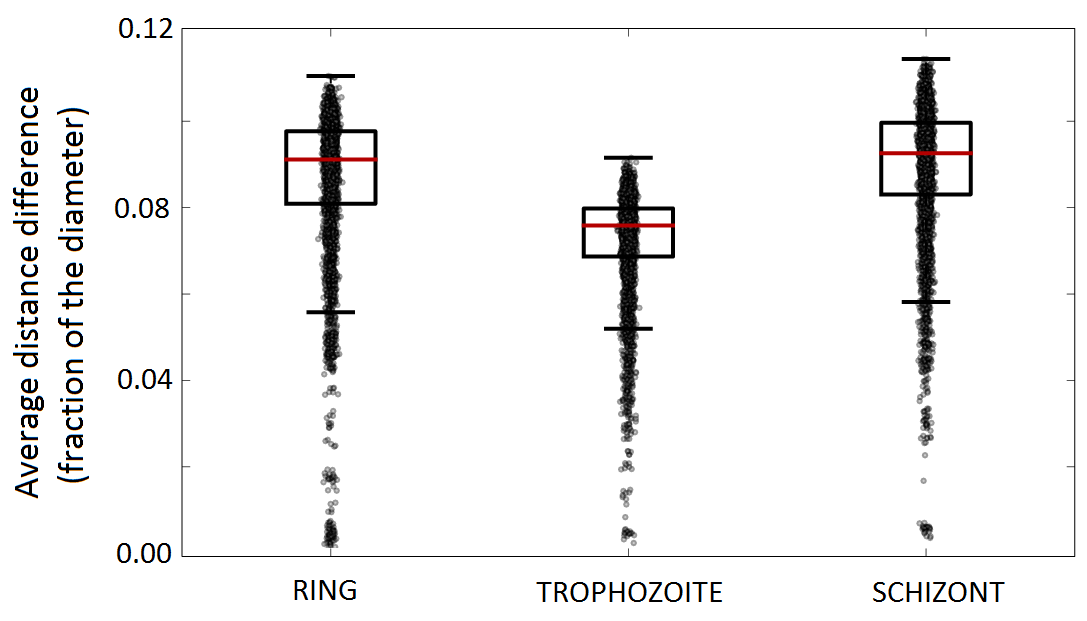
\includegraphics[width=0.8\textwidth]{suppFigs/stabilityOf3Dinference/compareStructurePairs.png}
   \end{center}
\caption{{\bf Similarity between 3D models inferred from 100 different initializations.}}
{We computed the average distance differences (Methods) for each pair of structures
(i.e., ${100 \choose 2}$) that are inferred from different initializations and
summarized these difference using a box plot for each stage. Each box extends from the
lower to upper quartile values with a red line at the median. These results show that
the 3D distance between a pair of loci varies, on the average, less than $10\%$ of the
nuclear diameter from one structure to another.
}
\label{suppfig:compareStructurePairs}
\end{figure}
\clearpage

% New fig
\begin{figure}
  \begin{center}
  \subfloat[Ring]{\includegraphics[width=0.85\textwidth]{suppFigs/3Dclustering/RINGS.pdf}} \hspace{0.15\textwidth}
  \subfloat[Trophozoite]{\includegraphics[width=0.85\textwidth]{suppFigs/3Dclustering/TROPHOZOITES.pdf}}\hspace{0.15\textwidth}
  \subfloat[Schizont]{\includegraphics[width=0.85\textwidth]{suppFigs/3Dclustering/SCHIZONTS.pdf}}
   \end{center}
\caption{{\bf Clustering of the 100 structures using pairwise RMSD values.}}
{ To assess whether the 100 structures generated from different random initializations fall into 
discrete clusters we performed hierarchical clustering on the pairwise RMSD matrix of each 
stage. We computed and plotted the Calinski-Harabasz (CH) 
index \cite{calinski:dendrite} for each clustering while varying the number of clusters from 2 to 50. 
None of the stages exhibited a clear peak of the CH index, suggesting that the set of structures do not fall into discrete clusters.
}
\label{suppfig:CHindices}
\end{figure}
\clearpage


\begin{figure}
  \begin{center}
  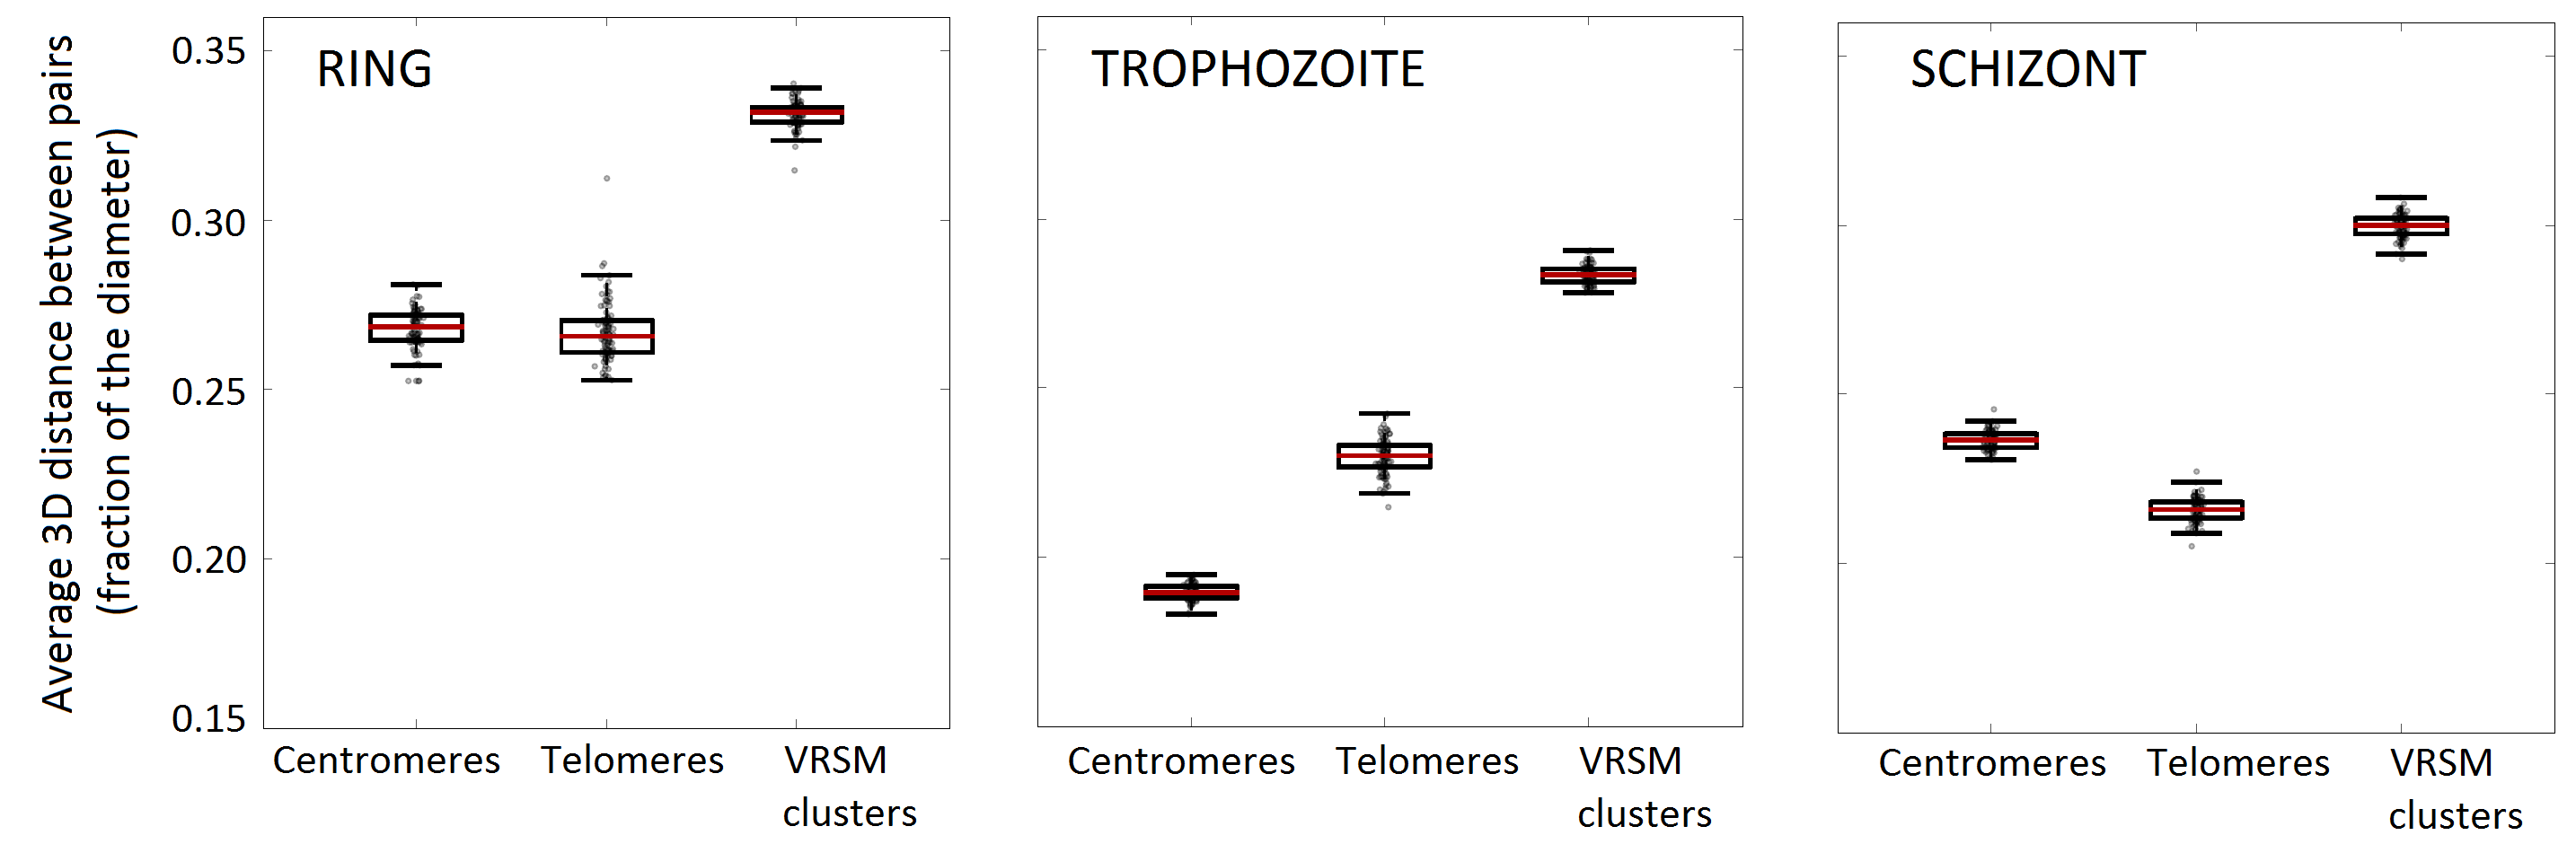
\includegraphics[width=1\textwidth]{suppFigs/stabilityOf3Dinference/allStages-clustering.png}
  \end{center}
\caption{{\bf Conservation of centromere, telomere and VRSM gene colocalizations across 100 different initializations. }}
{ We computed the average 3D distance between pairs of centromeres (${14 \choose 2}$ pairs),
telomeres (${28 \choose 2}$ pairs) and VRSM clusters (8 internal, 28 subtelomeric clusters and a total of ${36 \choose 2}$ pairs)
for each of the 100 structures inferred from different initializations and summarized
these average distances using a box plot for each stage. Each box extends from the
lower to upper quartile values with a red line at the median.  These results suggest that
the major organizational hallmarks concerning colocalization of centromere, telomere and
VRSM gene regions are common to all structures gathered from different initializations.}
\label{suppfig:clusteringIn100Structures}
\end{figure}
\clearpage




\begin{figure}
  \begin{center}
  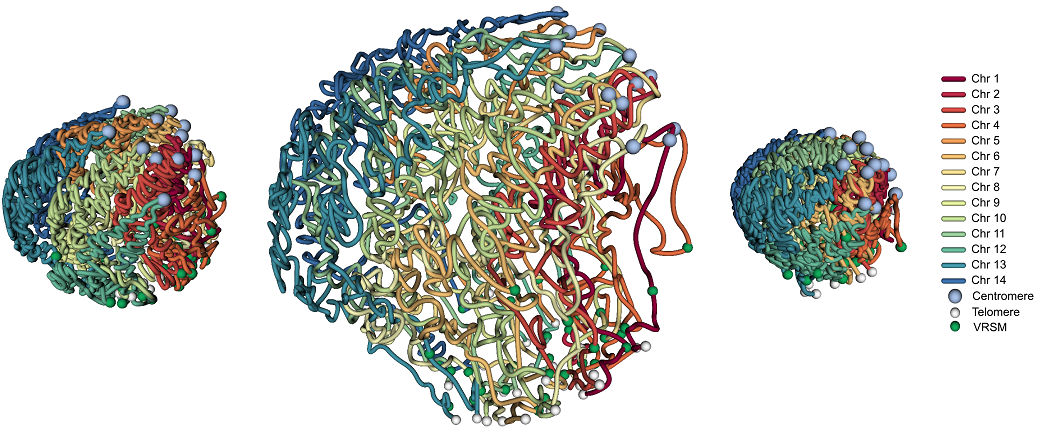
\includegraphics[width=1\textwidth]{suppFigs/3Dall/all3D-centromeres-angle-lowRes.png}
   \end{center}
\caption{{\bf 3D structures of all three stages (centromere clustering).}}
{This figure is identical to Main Figure 2a except the view is rotated to visualize the centromere
clustering for each stage. Centromeres and telomeres are indicated with light blue and white spheres,
respectively. Midpoints of VRSM gene clusters are shown with green spheres.}
\label{suppfig:3Dcentromeres}
\end{figure}
\clearpage


\begin{figure}
  \begin{center}
  \subfloat[Before clustering (Ring)]{\includegraphics[width=0.325\textwidth]{suppFigs/clusteringComparmentDists/RINGS.pdf}} \hspace{0.04\textwidth}
  \subfloat[Hierarchical clustering (Ring)]{\includegraphics[width=0.43\textwidth]{suppFigs/clusteringComparmentDists/RINGS-hierCluster-dists.pdf}} \hspace{0.1\textwidth}
  \subfloat[Before clustering (Trophozoite)]{\includegraphics[width=0.325\textwidth]{suppFigs/clusteringComparmentDists/TROPHOZOITES-XL.pdf}} \hspace{0.04\textwidth}
  \subfloat[Hierarchical clustering (Trophozoite)]{\includegraphics[width=0.43\textwidth]{suppFigs/clusteringComparmentDists/TROPHOZOITES-XL-hierCluster-dists.pdf}} \hspace{0.1\textwidth}
  \subfloat[Before clustering (Schizont)]{\includegraphics[width=0.325\textwidth]{suppFigs/clusteringComparmentDists/SCHIZONTS.pdf}} \hspace{0.04\textwidth}
  \subfloat[Hierarchical clustering (Schizont)]{\includegraphics[width=0.43\textwidth]{suppFigs/clusteringComparmentDists/SCHIZONTS-hierCluster-dists.pdf}}
  \end{center}
\caption{{\bf Hierarchical clustering of compartment distance matrices. }}
{Pairwise compartment distance matrices ($42\times42$, three compartments on each chromosome) that are identified
    by eigenvalue decomposition (Methods) for (a) ring, (c) trophozoite and (e) schizont stages. Distances are
    averaged over all pairs of loci between the two compartments and normalized using nuclear diameter to result
    in a fraction between 0 and 1. In the figure, the actual length of each compartment and each chromosome are preserved.
    Each compartment is colored separately, with dashed lines segregating adjacent chromosomes.
    Hierarchical clustering of pairwise compartment distance matrices for (b) ring, (d) trophozoite and
    (f) schizont stages. Clustering was performed using the average linkage score.
    Each compartment is represented by a fixed length, and L, M, R denote left, mid, right
    compartments, respectively. For all panels the color bars extend from 0 to 0.5
    (i.e., distance equals nuclear radius).
}
\label{suppfig:compDists}
\end{figure}
\clearpage

\begin{figure}
  \begin{center}
  \subfloat[]{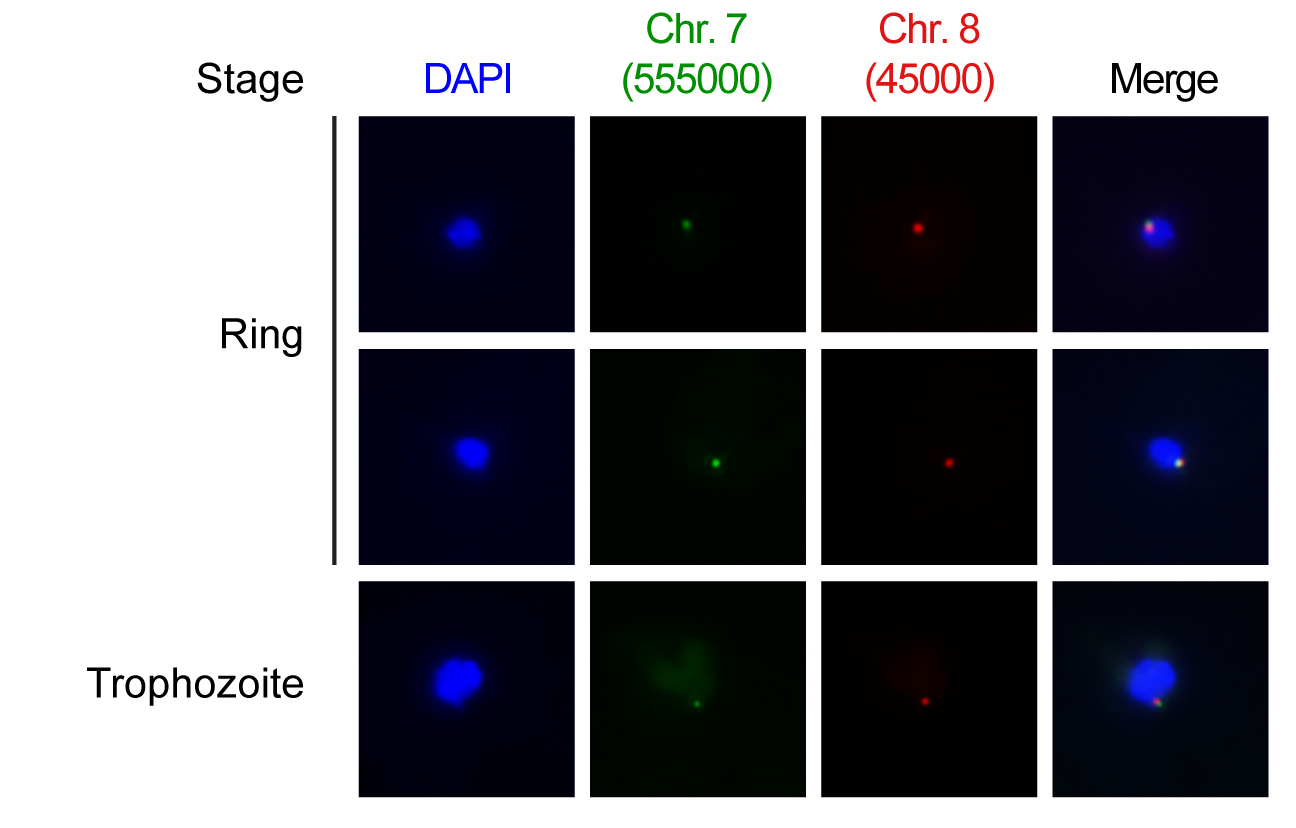
\includegraphics[width=0.69\textwidth]{suppFigs/FISH/varPair.png}} \\
  \subfloat[]{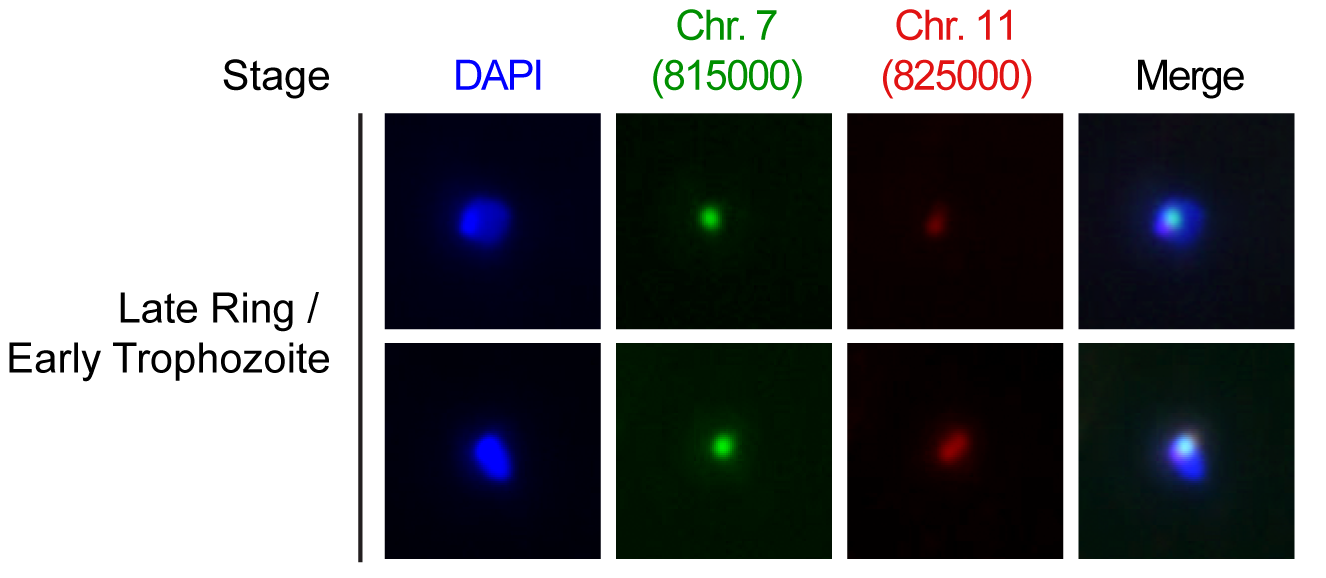
\includegraphics[width=0.69\textwidth]{suppFigs/FISH/nonvarPair.png}} \\
  \hspace{0.015\textwidth}
  \subfloat[]{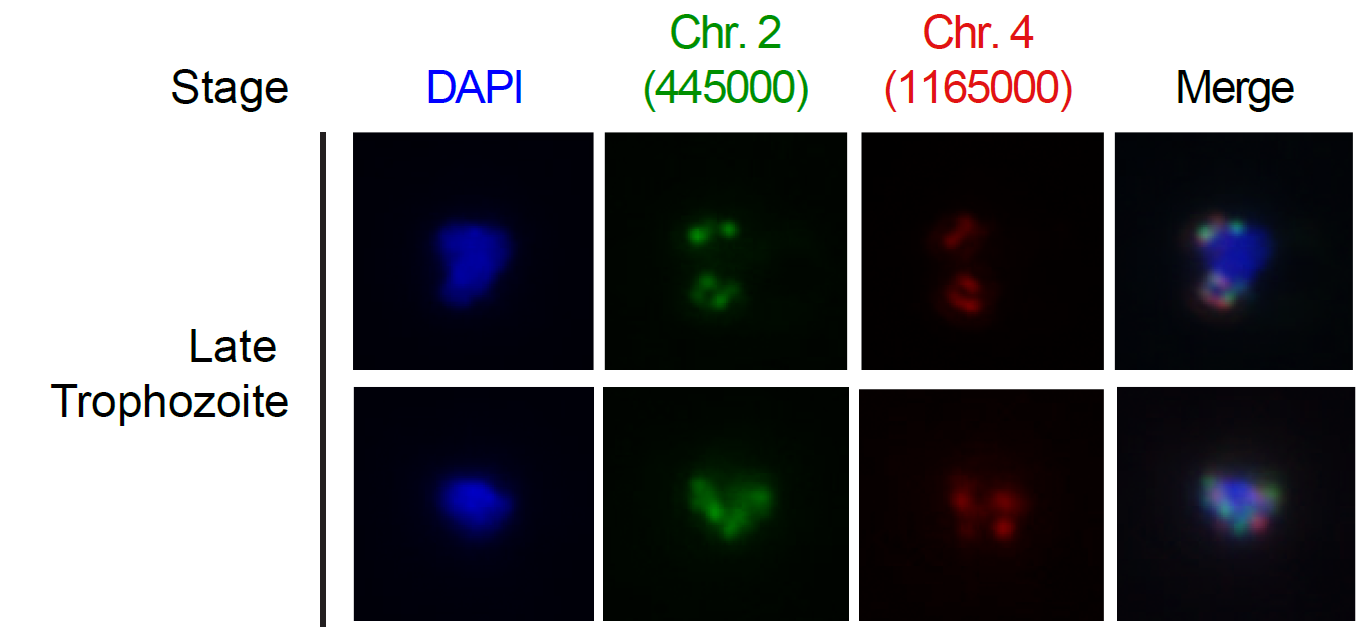
\includegraphics[width=0.65\textwidth]{suppFigs/FISH/controlPair.png}}\\
  \end{center}
\caption{{\bf Validation of 3D models with DNA FISH.}}
{ Additional FISH images for (a) a pair of interchromosomal loci with VRSM
  genes (chr7:550,000-560,000 containing internal VRSM genes and
  chr8:40,000-50,000 containing subtelomeric VRSM genes)
  (b) a pair of interchromosomal loci that harbor no VRSM genes
  (chr7:810,000-820,000 and chr11:820,000-830,000).
  (c) FISH images showing lack of colocalization as a negative
  control for a pair of interchromosomal loci that harbor no VRSM genes
  and have no contacts in trophozoite stage (chr2:440,000-450,000 and chr4:1,160,000-1,170,000).
}
\label{suppfig:fish}
\end{figure}
\clearpage

\begin{figure}
  \begin{center}
%  \subfloat[Our data - Ring]{\includegraphics[width=0.32\textwidth]{suppFigs/Newbold-virtual4Cs/RINGS/chr7-rDNA/chr5.pdf}} \hspace{0.05\textwidth}
%  \subfloat[Our data - Trophozoite]{\includegraphics[width=0.32\textwidth]{suppFigs/Newbold-virtual4Cs/TROPHOZOITES-XL/chr7-rDNA/chr5.pdf}} \vspace{-0.01\textwidth}
%  \subfloat[Our data - Schizont]{\includegraphics[width=0.32\textwidth]{suppFigs/Newbold-virtual4Cs/SCHIZONTS/chr7-rDNA/chr5.pdf}} \hspace{0.05\textwidth}
%  \subfloat[Our data - Trophozoite control]{\includegraphics[width=0.32\textwidth]{suppFigs/Newbold-virtual4Cs/TROPHOZOITES-NL/chr7-rDNA/chr5.pdf}}
%  \vspace{-0.01\textwidth}
%	
  \subfloat[Lemieux et al. data - DCJ
  On]{\includegraphics[width=0.32\textwidth]{suppFigs/Newbold-virtual4Cs/\detokenize{DCJ_On-HiC-MboI}/chr7-rDNA/chr5.pdf}} \hspace{0.05\textwidth}
  \subfloat[Lemieux et al. data - DCJ
  Off]{\includegraphics[width=0.32\textwidth]{suppFigs/Newbold-virtual4Cs/\detokenize{DCJ_Off-HiC-MboI}/chr7-rDNA/chr5.pdf}} \vspace{-0.01\textwidth}
  \subfloat[Lemieux et al. data - B15C2]{\includegraphics[width=0.32\textwidth]{suppFigs/Newbold-virtual4Cs/B15C2-HiC-MboI/chr7-rDNA/chr5.pdf}}
  \hspace{0.05\textwidth}
  \subfloat[Lemieux et al. data - NF54 control]{\includegraphics[width=0.32\textwidth]{suppFigs/Newbold-virtual4Cs/NF54-Control-MboI/chr7-rDNA/chr5.pdf}}
  \end{center}
\caption{{\bf Clustering of highly transcribed rDNA units in Lemieux et al. data.}}
{Hi-C libraries generated with MboI restriction enzyme
    from Lemieux et al. \cite{lemieux:genome-wide}  were mapped
    to the \emph{P. falciparum} genome and further processed using the
    pipeline we processed our data with to generate and normalize contact maps at 25 kb resolution.
    The normalized contact maps were used for virtual 4C plots using as a bait
    the A-type rDNA unit on chromosome 7. As suggested in Lemieux et al.,
    contact counts from 50 kb up- and downstream of the 25 kb bin containing
    rDNA unit were used, and the rDNA-containing window itself was removed
    from the analysis. For each window $w$ on chromosome 5, the contact
    enrichment was calculated by dividing the contact count between
    the bait and $w$ to the average interchromosomal contact count for
    the bait locus.
}
\label{suppfig:rDNAunitsOn3D}
\end{figure}
\clearpage



\begin{figure}
\begin{center}
\subfloat{
    \begin{tabular}{ccc}
      \includegraphics[width=0.33\textwidth]{suppFigs/intraVSinter/per10kb-B15C2-HiC-MboI.pdf}  & \hspace{0.1\textwidth} & \includegraphics[width=0.33\textwidth]{suppFigs/intraVSinter/equalOcc-B15C2-HiC-MboI.pdf} \\
      (a) Lemieux et al. data - B15C2 & \hspace{0.1\textwidth} & (b) Lemieux et al. data - B15C2 \\
      & & \\
        \includegraphics[width=0.33\textwidth]{suppFigs/intraVSinter/equalOcc-RINGS.pdf}	& \hspace{0.1\textwidth} & \includegraphics[width=0.33\textwidth]{suppFigs/intraVSinter/equalOcc-TROPHOZOITES-XL.pdf} \\
		(c) Our data - Ring & \hspace{0.1\textwidth} & (d) Our data  - Trophozoite\\
      & & \\
        \multicolumn{3}{c}{\includegraphics[width=0.33\textwidth]{suppFigs/intraVSinter/equalOcc-SCHIZONTS.pdf}} \\
		\multicolumn{3}{c}{(e) Our data - Schizont}
    \end{tabular}
}
\end{center}
\caption{{\bf Comparison of inter and intrachromosomal contact prevalence. }}
{ The relationship between contact count and genomic distance is estimated
    using bins with equal genomic distances (e.g., 10 kb, 20 kb) in Lemieux
    et al. \cite{lemieux:genome-wide}. Due to the diminishing number of possible
    locus pairs with increasing genomic distance (e.g., only one locus pair for
    the bin with the largest genomic distance) this estimation leads to many
    high variance bins for large genomic distances. This issue can be addressed
    by using variable-width bins that contain equal numbers of
    contacts (see Methods). Plotted are the $\log$ (base $e$) of mean
    contact count per bin when using (a) equal distance binning, (b)
    equal occupancy binning for B15C2 library of Lemieux et
    al. \cite{lemieux:genome-wide} and (c-e) equal occupancy binning for
    ring, trophozoite and schizont stage data from this work. Dashed vertical
    red lines denote the range used to compute the log-linear fit.
}
\label{suppfig:intraVSinter}
\end{figure}
\clearpage

\begin{figure}
  \begin{center}
  \includegraphics[width=0.8\textwidth]{suppFigs/chrTerritory/diam2point5.pdf}
   \end{center}
\caption{{\bf Changes in chromosome territories during the erythrocytic cycle.}}
{ The extent to which a chromosome intermingles with other chromosomes is
    characterized by the percentage of nuclear volume that is jointly occupied
    by the chromosome of interest and at least one other chromosome,
    relative to the entire volume occupied by the chromosome.
    To compute the percentages on the y-axis, the nuclear volume was sampled using
    1,000,000 randomly generated small spheres with radius 5\% of the actual nuclear
    radius. For each chromosome $i$, two numbers were calculated: the number of spheres that contain a locus
    from chromosome $i$ ($n_i$) and the number of such spheres that
    contain no locus from another chromosome ($e_i$). The percent intermingled (y-axis)
    for chromosome $i$ is computed as $100\times \frac{n_i-e_i}{n_i}$.
    Because the exact percentages are highly dependent on the selection of the random
    sphere size, the procedure was repeated using spheres with
    radii 2\%, 10\% and 20\% of the nuclear volume.  For each setting,
    the trophozoite stage exhibited the highest amount of intermingling,
    whereas the schizont stage showed the lowest. Also, the
    larger chromosomes (i.e., chromosomes with higher numbers)
    consistently showed lower intermingling compared to smaller
    chromosomes at each stage and for each threshold.}
\label{suppfig:territory}
\end{figure}
\clearpage


\begin{figure}
  \begin{center}
%  \subfloat[]{\includegraphics[width=0.55\textwidth]{suppFigs/clusteringComparmentDists/RINGS.png}}
  \subfloat[From ring to trophozoite]{\includegraphics[width=0.6\textwidth]{suppFigs/clusteringComparmentDists/RINGS-minus-TROPHOZOITES-XL.pdf}}
  \hspace{0.03\textwidth}
%  \subfloat[]{\includegraphics[width=0.55\textwidth]{suppFigs/clusteringComparmentDists/TROPHOZOITES-XL.png}}
  \subfloat[From trophozoite to schizont]{\includegraphics[width=0.6\textwidth]{suppFigs/clusteringComparmentDists/TROPHOZOITES-XL-minus-SCHIZONTS.pdf}}
%  \subfloat[]{\includegraphics[width=0.55\textwidth]{suppFigs/clusteringComparmentDists/SCHIZONTS.png}}
%  \subfloat[]{\includegraphics[width=0.55\textwidth]{suppFigs/clusteringComparmentDists/SCHIZONTS-hierCluster-dists.png}}
  \end{center}
\caption{{\bf Movement of chromosome compartments with respect to each other.}}
{ Each compartment movement matrix is generated by subtracting the pairwise compartment
    distance matrix (Supplementary Fig. \ref{suppfig:compDists}) of one stage from the
    matrix of the preceding stage. Plotted are the movements (a) from ring to trophozoite
    (i.e., trophozoite minus ring), (b) from trophozoite to schizont (i.e.,  schizont minus
    trophozoite). Red color indicates that a pair of compartments are closer in the later
    stage compared to the earlier, and blue color indicates vice versa.
}
\label{suppfig:compMovement}
\end{figure}
\clearpage


\begin{figure}
  \begin{center}
  \subfloat[]{\includegraphics[width=0.7\textwidth]{suppFigs/VE/correlation-per-num-experiments.png}}
  \hspace{0.03\textwidth}
  \subfloat[]{
  \begin{tabular}{llcccc}
    \hline
    \emph{Contact map 1} & \emph{Contact map 2} & \emph{Row-based corr.} & \emph{Normalized row-based corr.}   \\
    \hline
    \multirow{2}{*}{Yeast \textit{(Hi-C)\cite{duan:three}}} &Yeast \textit{(VE)} & 0.915 & 0.573 \\
    & Yeast \textit{(expected)} & 0.922 & 0.115 \\\hline
    \multirow{2}{*}{Ring \textit{(Hi-C)}} &Ring \textit{(VE)} & 0.843 & 0.340 \\
    & Ring \textit{(expected)} & 0.928 & 0.072 \\\hline
    \multirow{2}{*}{Trophozoite \textit{(Hi-C)}} &Trophozoite \textit{(VE)} & 0.848 & 0.392 \\
    & Trophozoite \textit{(expected)} & 0.908 & 0.063 \\\hline
    \multirow{2}{*}{Schizont \textit{(Hi-C)}} &Schizont \textit{(VE)} & 0.864 & 0.487 \\
    & Schizont \textit{(expected)} & 0.923 & 0.081 \\
    \hline
    \end{tabular}}
  \end{center}
\caption{{\bf Volume exclusion modeling and correlation calculation.}}
{ (a) Row-based Pearson correlation between the observed Hi-C contact map
    and the average contact map from volume exclusion modeling as a function
    of the number of simulated structures.
    (b) Row-based Pearson correlation and normalized row-based Pearson
    correlation between the two contact maps listed in each row for
    various Hi-C libraries. \emph{VE} refers to
    contact maps obtained from 5000 structures generated by volume exclusion
    and \emph{expected} refers to matrices with expected contact counts
    generated from observed \emph{Hi-C} matrices as described in Methods.
    }
\label{suppfig:VEconvergence}
\end{figure}
\clearpage


\begin{figure}
\begin{center}
\subfloat[]{\includegraphics[width=3in]{suppFigs/TADs/TAD-descriptive.png}}
\hspace{0.03\textwidth}
\subfloat[]{\begin{tabular}{lccccc}
\hline
%\multirow{2}{*} {\emph{Internal VRSM}} & \multirow{2}{*}{\emph{Stage}} & \multirow{2}{*}{Mean($\frac{t_2-t_1}{t_2+t_1}$)} & \multirow{2}{*}{Mean($\frac{t_2-t_3}{t_2+t_3}$)} & \multirow{2}{*}{Mean($\frac{r_5-r_4}{r_5+r_4}$)} & \multirow{2}{*}{Mean($\frac{r_6-r_7}{r_6+r_7}$)} \\
%& & & & &\\\hline
%% OR
\emph{Internal VRSM} & \emph{Stage} & $t_2$ vs. $t_1$ & $t_2$
vs. $t_3$ & $r_5$ vs. $r_4$ & $r_6$ vs. $r_7$ \\ \hline
\multirow{3}{*} {chr4(1)}	&	R	&	\cellcolor[gray]{0.8}0  &	0.7  &  \cellcolor[gray]{0.8}0  &  -0.09 \\
	&	T	&	0.06	&	0.2  &  -0.11  &  -0.25 \\
	&	S	&	0.1  &	0.16  &  \cellcolor[gray]{0.8}0.13  &  -0.14 \\\hline
\multirow{3}{*} {chr4(2)}	&	R	&	0.13	&	0.12  &  -0.38  &  -0.27 \\
	&	T	&	0.15	&	0.15  &  -0.42  &  -0.33 \\
	&	S	&	0.14	&	0.13  &  -0.37  &  -0.3 \\\hline
\multirow{3}{*} {chr4(3)}	&	R	&	0.03	&	0.08  &  -0.37  &  -0.34 \\
	&	T	&	0.03	&	0.06  &  -0.55  &  -0.41 \\
	&	S	&	0.03	&	0.01  &  -0.48  &  -0.42 \\\hline
\multirow{3}{*} {chr6(1)}	&	R	&	0.12	&	0.1  &  \cellcolor[gray]{0.8}0.02  &  -0.06 \\
	&	T	&	0.19	&	0.2  &  -0.09  &  -0.16 \\
	&	S	&	0.16	&	0.18  &  -0.08  &  -0.14 \\\hline
\multirow{3}{*} {chr7(1)}	&	R	&	0.11	&	0.2  &  -0.19  &  -0.18 \\
	&	T	&	0.19	&	0.28  &  -0.36  &  -0.3 \\
	&	S	&	0.08	&	0.19  &  -0.27  &  -0.27 \\\hline
\multirow{3}{*} {chr8(1)}	&	R	&	0.15	&	0.08  &  -0.05  &  -0.09 \\
	&	T	&	0.17	&	0.09  &  -0.17  &  -0.13 \\
	&	S	&	0.14	&	0.09  &  -0.11  &  -0.11 \\\hline
\multirow{3}{*} {chr12(1)}	&	R	&	0.07	&	0.05  &  -0.02  &  -0.01 \\
	&	T	&	0.05	&	0.14  &  -0.04  &  -0.02 \\
	&	S	&	0.09	&	0.12  &  -0.07  &  -0.08 \\\hline
\multirow{3}{*} {chr12(2)}	&	R	&	0.09	&	0.09  &  -0.09  &  -0.11 \\
	&	T	&	0.17	&	0.1  &  -0.27  &  -0.24 \\
	&	S	&	0.09	&	0.07  &  -0.19  &  -0.23 \\\hline
\end{tabular}
}
\end{center}
\caption{{\bf Quantification of domain-like behavior of VRSM gene
    clusters.}} {(a) Each internal VRSM gene cluster is characterized
  by a set of strong intra-cluster contacts ($t_2$) and two sets of
  contacts with adjacent regions ($r_5$ and $r_6$) that are weak. For
  comparison, we also consider flanking, non-VSRM regions of the same
  size as the original VRSM cluster, including their ``intra-cluster''
  contacts ($t_1$ and $t_3$) which should be similar to $t_2$ for
  a contact map without domain-like structures around VRSM clusters
  and contacts with adjacent regions ($r_4$ and $r_7$) which are
  comparable to ($r_5$ and $r_6$). As seen in this example,
  a domain-like structure for a VRSM cluster leads to stronger
  contacts (+ sign) within $t_2$ compared to both $t_1$ and $t_3$, and weaker
  contacts (- sign) within $r_4$ and $r_7$ compared to $r_5$ and $r_6$.
  (b) The table reports, for each internal
  VRSM gene cluster and each stage, the average normalized difference between
  the intra-cluster contacts within the cluster compared to its
  two flanking control regions, and similarly for the contacts
  with adjacent regions.  The metric we use for comparing two contact
  sub-matrices $X$, $Y$ of
  dimension $N \times M$ is $\frac{1}{NM} \sum_{i=1}^N \sum_{j=1}^M
  \frac{x_{ij} - y_{ij}}{\frac{1}{2}(x_{ij}+y_{ij})}$ where $x_{ij}$ and
  $y_{ij}$ are the $ij$th entries of $X$ and $Y$, respectively.
  Values that have signs inconsistent with the expected pattern
  (i.e., +, +, -, -) are indicated with a grey background. Every internal
  VRSM cluster exhibits the expected sign pattern in at least one stage.
  }
\label{suppfig:TADs}
\end{figure}
\clearpage

\begin{figure}
  \begin{center}
  \subfloat[All genes]{\includegraphics[width=0.45\textwidth]{suppFigs/expVSdists/all-corr-contactCounts.pdf}}
  \hspace{0.05\textwidth}
  \subfloat[Excluding VRSM genes]{\includegraphics[width=0.45\textwidth]{suppFigs/expVSdists/all-corr-contactCounts-withoutVRSM.pdf}}
  \hspace{0.05\textwidth}
  \subfloat[All genes]{\includegraphics[width=0.45\textwidth]{suppFigs/expVSdists/all-100-3Ddists.pdf}}
  \hspace{0.05\textwidth}
  \subfloat[Excluding VRSM genes]{\includegraphics[width=0.45\textwidth]{suppFigs/expVSdists/all-100-3Ddists-withoutVRSM.pdf}}
%  \hspace{0.05\textwidth}
%  \subfloat[All genes]{\includegraphics[width=0.45\textwidth]{suppFigs/expVSdists/all-corr.pdf}}
%  \hspace{0.05\textwidth}
%  \subfloat[Excluding VRSM genes]{\includegraphics[width=0.45\textwidth]{suppFigs/expVSdists/all-corr-withoutVRSM.pdf}}
   \end{center}
\caption{{\bf Revisiting the relationship between 3D architecture and gene expression by excluding VRSM genes. }}
{   (a) is identical to Main Figure 6a and (b) is generated identical to (a) except all gene pairs
    involving at least one VRSM gene are omitted from the analysis. Re-evaluation of our
    hypothesis that interchromosomal gene pairs that have contact counts within the top 20\%
    for each stage have more highly correlated expression profiles than the remaining gene pairs
    still yielded significant p-values for each stage [Wilcoxon rank-sum test, p-values 1.07e-70 (ring),
    0 (trophozoite), and 1.68e-302 (schizont)].
    (c) is identical to Main Figure 6b and (d) is generated identical to (c) except all gene pairs
    involving at least one VRSM gene are omitted from the analysis. Re-evaluation of our
    hypothesis that interchromosomal gene pairs closer than 20\% of the nuclear diameter have more
    highly correlated expression profiles than other genes still yielded
    significant p-values for each stage [Wilcoxon rank-sum test, p-values 3.27e-48 (ring),
    1.32e-157 (trophozoite), and 2.16e-5 (schizont)].
}
\label{suppfig:expVSdistWithoutVRSM}
\end{figure}
\clearpage

\begin{figure}
  \begin{center}
  \subfloat[All genes]{\includegraphics[width=0.45\textwidth]{suppFigs/expVSdists/telomeres-100-corr.pdf}}
  \hspace{0.05\textwidth}
  \subfloat[Excluding VRSM genes]{\includegraphics[width=0.45\textwidth]{suppFigs/expVSdists/telomeres-100-corr-withoutVRSM.pdf}}
  \hspace{0.05\textwidth}
  \subfloat[All genes]{\includegraphics[width=0.45\textwidth]{suppFigs/expVSdists/centromeres-100-corr.pdf}}
  \hspace{0.05\textwidth}
  \subfloat[All genes]{\includegraphics[width=0.45\textwidth]{suppFigs/expVSdists/center-100-corr.pdf}}
   \end{center}
\caption{{\bf The relationship between distance to the telomeres, nuclear center and centromeres versus the gene expression.}}
{   (a) is identical to Main Figure 6c and (b) is generated identical to (a) except
    all VRSM genes are omitted from the analysis.
    Re-evaluation of our hypothesis that genes which lie within a distance of
    20\% of the nuclear diameter to the centroid of the telomeres exhibit lower expression
    levels yielded a significant p-value for trophozoite stage but not for ring and
    schizont stages at a significance threshold of $0.01$ [Wilcoxon rank-sum test,
    p-values 0.21 (ring), 1.5e-3 (trophozoite), and 0.035 (schizont)].
    (c) and (d) are generated identical to (a) expect the distance of genes are measured to
    (c) the centroid of the centromeres and (d) the nuclear center.
    For each figure, genes are first sorted in increasing order according to their distances
    to the landmark of interest and then binned into 20 equal width quantiles
    ($5$th, $10$th, ..., $100$th). For each bin, the average distance to the landmark (x-axis)
    and the average log expression value~\citep{bunnik:polysome} together with its standard
    error (y-axis) are computed and plotted.
}
\label{suppfig:distToCenter}
\end{figure}
\clearpage


\begin{figure}
\begin{center}
\subfloat{
    \begin{tabular}{ccc}
      \includegraphics[width=0.28\textwidth]{suppFigs/kCCA/RINGS-kcca-genes-1.png} & \hspace{0.1\textwidth} & \includegraphics[width=0.28\textwidth]{suppFigs/kCCA/RINGS-kcca-genes-2.png} \\
      (a) First component (Ring) & \hspace{0.1\textwidth} & (b) Second component (Ring) \\
     % & & \\
        \includegraphics[width=0.28\textwidth, angle=-165]{suppFigs/kCCA/TROPH-kcca-genes-1.png} & \hspace{0.1\textwidth} & \includegraphics[width=0.28\textwidth, angle=-165]{suppFigs/kCCA/TROPH-kcca-genes-2.png} \\
      (c) First component (Trophozoite) & \hspace{0.1\textwidth} & (d) Second component (Trophozoite) \\
      %& & \\
        \includegraphics[width=0.28\textwidth, angle=-25]{suppFigs/kCCA/SCHIZONTS-kcca-genes-1.png} & \hspace{0.1\textwidth} & \includegraphics[width=0.28\textwidth, angle=-25]{suppFigs/kCCA/SCHIZONTS-kcca-genes-2.png} \\
      (e) First component (Schizont) & \hspace{0.1\textwidth} & (f) Second component (Schizont) \\
      %& & \\
      \multicolumn{3}{c}{\includegraphics[width=0.3\textwidth]{suppFigs/kCCA/legend.png}} \\
    \end{tabular}
}
\end{center}
\caption{{\bf kCCA expression profiles component score.}}  { Each
  panel shows the projection of the gene expression profile onto one
  of the two extracted kCCA profiles for a specified erythrocytic
  stage, with the score of the projection encoded on the color
  scale. For the first kCCA component, the projections consistently
  exhibit a striking gradient from the telomeric region across
  the nucleus, while for the second component, which is less coherent
  with the 3D structure, the projection gradient extends from the
  centromeres across the nucleus.  }
\label{suppfig:kCCAsecond}
\end{figure}
\clearpage


% ================== FIGURES THAT MAY NOT END UP BEING REFERRED TO ==================



% ================================================================================
% SUPPLEMENTARY METHODS
\section*{Supplementary Notes}
%\addcontentsline{toc}{section}{Supplementary Results}
\phantomsection

\addcontentsline{toc}{subsection}{{\bf 1} \indent {\bf Tethered conformation capture procedure protocol}}
\subsection*{Supplementary Note 1: Tethered conformation capture procedure}
\label{supp:ourHiC}
\paragraph{Day 1}
 Parasite pellets were thawed on
ice in 550 $\mu$l Hi-C lysis buffer (25 mM Tris-HCl at pH 8.0, 10 mM NaCl,
2 mM AEBSF, Roche Complete Mini EDTA-free protease inhibitor cocktail
[Roche, Basel, Switzerland], 0.25\% Igepal CA-630) per 140
mg. Parasite membranes were disrupted by passing the lysate through a
26.5 gauge needle 15 times using a syringe. Samples were spun at 2,500
$\times$ g for 5 min at room temperature (RT). Pellets were washed twice with
1 ml ice-cold wash buffer (50 mM Tris-HCl at pH 8.0, 50 mM NaCl, 1 mM
EDTA) and resuspended in the same buffer to a final volume of 250
$\mu$l. Samples were mixed with 95 $\mu$l 2\% SDS to a final concentration of
0.5\% and incubated at 55$^\circ$C for 15 min. Suspensions were cooled down
to RT before they were mixed with 105 $\mu$l 25 mM EZ-link
Iodoacetyl-PEG2-Biotin (IPB) (Thermo Fisher Scientific, Waltham, MA,
USA) to biotinylate proteins. After incubating for 1 h at RT while
rotating, the SDS was neutralized by adding 1.3 ml 1$\times$ NEBuffer 2 (New
England Biolabs [NEB], Ipswich, MA, USA). Samples were mixed with 225
$\mu$l 10\% Triton X-100 to a final concentration of 1\% and incubated for
10 min on ice, followed by 10 min at 37$^\circ$C. Five $\mu$l 1 M DTT, 100 $\mu$l 10$\times$
NEBuffer 2, 415 $\mu$l water and 35 $\mu$l MboI restriction enzyme (NEB) (25
units/$\mu$l) was added to digest the DNA overnight at 37$^\circ$C in a total
volume of 2,530 $\mu$l.

\paragraph{Day 2}
After digestion, samples were loaded into a Slide-A-Lyzer Dialysis
Cassette G2 (Thermo Fisher Scientific) and dialyzed for 4 h at RT
against 1 L of dialysis buffer (10 mM Tris-HCl at pH 8.0, 1 mM EDTA)
to eliminate excess IPB remaining from the biotinylation
step. Dialysis buffer was renewed after 3 h. Four hundred $\mu$l MyOne
Streptavidin T1 beads (Life Technologies, Carlsbad, CA, USA) were
washed 3 times with PBS + 0.01\% Tween-20 (PBST) and beads were
resuspended in 2 ml PBST. Dialyzed samples were divided into 5 equal
aliquots of 500 $\mu$l in 1.7 ml prelubricated microcentrifuge tubes
(Corning, Corning, NY, USA). Four hundred $\mu$l beads were added to each
tube and samples were incubated for 30 min at RT while rotating. To
prevent interference of unbound streptavidin on the beads with later
steps (adding biotinylated dCTP) 5 $\mu$l neutralized IPB was added to
each tube. IPB was neutralized by adding an equimolar amount of
2-mercaptoethanol. Samples were incubated for an additional 15 min at
RT while rotating. Not biotinylated chromatin and not cross-linked DNA
was removed by washing the magnetic T1 beads once with 600 $\mu$l PBST and
once with 600 $\mu$l wash buffer (10 mM Tris-HCl at pH 8.0, 50 mM NaCl,
0.4\% Triton X-100). Beads were resuspended in 100 $\mu$l of the same wash
buffer. MboI generated $5'$ overhangs were filled in by adding 63 $\mu$l
water, 1 $\mu$l 1 M MgCl, 10 $\mu$l 10$\times$ NEBuffer 2, 0.7 $\mu$l 10 mM dATP, 0.7 $\mu$l
10 mM dTTP, 0.7 $\mu$l 10 mM 2'-Deoxyguanosine-5'-O-(1-thiotriphosphate),
sodium salt, Sp-isomer (Axxora, San Diego, CA, USA), 15 $\mu$l 0.4 mM
Biotin-14-dCTP (Life Technologies), 4 $\mu$l 10\% Triton X-100 and 5 $\mu$l
5U/$\mu$l DNA Polymerase I, Large (Klenow) Fragment (NEB). Samples were
incubated for 40 min at RT while rotating. Reaction was stopped by
adding 5 $\mu$l 0.5 M EDTA to the suspension. After 2 min of incubation at
RT while rotating, beads were washed twice with 600 $\mu$l buffer (50 mM
Tris-HCl at pH 7.4, 0.4\% Triton X-100, 0.1 mM EDTA) and resuspended
in 500 $\mu$l of the same buffer. Each sample was transferred into a 15 ml
centrifuge tube. For blunt-end ligation under dilute conditions 500 $\mu$l
sample was mixed with 4 ml water, 250 $\mu$l 10$\times$ Ligase Buffer (NEB), 100
$\mu$l 1 M Tris-HCl at pH 7.4, 90 $\mu$l 20\% Triton X-100, 50 $\mu$l 100$\times$ BSA and
2 $\mu$l 2,000 U/$\mu$l T4 DNA Ligase (NEB), and incubated overnight at 16$^\circ$C.

\paragraph{Day 3}
The ligation reaction was stopped by adding 200 $\mu$l 0.5 M EDTA to each
of the five 15 ml tubes. The magnetic T1 beads were collected on the
wall of the tube using a magnet and the solution was aspirated out of
the tube. The beads were resuspended in 400 $\mu$l extraction buffer (50
mM Tris-HCl at pH 8.0, 0.2\% SDS, 1 mM EDTA, 500 mM NaCl) and the mix
was transferred into a new microcentrifuge tube. Samples were treated
with 5 $\mu$l RNase A (20 mg/ml) (Life Technologies) for 45 min at 37$^\circ$C
and with 20 $\mu$l Proteinase K (20 mg/ml) (NEB) overnight at 45$^\circ$C.

\paragraph{Day 4}
An additional 5 $\mu$l Proteinase K was added and samples were incubated
for another 2 h at 45$^\circ$C. Beads were collected on the wall of the tube
and DNA was extracted from the supernatant twice with an equal volume
of phenol:chloroform:isoamyl alcohol (25:24:1) and once with an equal
volume of chloroform. The aqueous phase was mixed with sodium chloride
and glycogen to a final concentration of 200 mM and 25 $\mu$g/ml,
respectively. DNA was precipitated by adding 900 $\mu$l ice-cold 200 proof
pure ethanol and incubation at -20$^\circ$C overnight or at -80$^\circ$C for
$>1$ h. Precipitated DNA was pelleted by centrifugation at 16,100 $\times$ g
for 30 min at 4$^\circ$C. Pellets were washed with ice-cold 80\% ethanol,
spun down at 16,100 $\times$ g for 15 min at 4$^\circ$C and resuspended in 20 $\mu$l 10
mM Tris-HCl at pH 8.0.

\paragraph{Day 5}
Two to five $\mu$g purified DNA was treated with Exonuclease III (NEB) (60
units per $\mu$g DNA) in 120 $\mu$l 1$\times$ NEBuffer 1 for one h at 37$^\circ$C. The
reaction was ended by adding 2.7 $\mu$l 0.5 M EDTA and 2.7 $\mu$l 5 M NaCl,
and subsequent incubation at 70$^\circ$C for 20 min. DNA was transferred into
TPX microtubes (Diagenode, Denville, NJ, USA) and sonicated using a
Bioruptor UCD-200 (Diagenode) at high intensity for 30 min using 30
sec on, 30 sec off cycles. Agencourt AMPure XP beads (Beckman Coulter,
Brea, CA, USA) were used to purify DNA, which was eluted in 50 $\mu$l
water.

\paragraph{Day 6}
All amounts mentioned for subsequent end-repair and adding of
A-overhangs are per $\mu$g of DNA used as input at the start of Day 5. DNA
ends were repaired by treating the DNA with 1 U of DNA Polymerase I,
Large (Klenow) Fragment (NEB), 3 U of T4 DNA Polymerase (NEB), 10 U of
T4 Polynucleotide Kinase (NEB) in 100 $\mu$l 1$\times$ T4 DNA Ligase Buffer (NEB)
with 0.4 mM of dNTPs for 30 min at 20$^\circ$C. Importantly, T4 DNA
Polymerase and not T4 DNA Ligase should be used for end-repair (Reza
Kalhor, personal communication). This was apparently written
incorrectly in the original TCC protocol \cite{kalhor:genome}. DNA was purified using
magnetic beads and eluted in 40 $\mu$l water. A-overhangs were added by
treating the DNA with 3 U of Klenow Fragment ($3' \rightarrow 5'$ exo--) (NEB) in 50
$\mu$l 1$\times$ NEBuffer 2 with 0.2 mM dATP for 30 min at 37$^\circ$C. The reaction was
ended by adding 1 $\mu$l of 0.5 M EDTA. Ten $\mu$l of MyOne Streptavidin C1
magnetic beads (Invitrogen) were washed twice with 500 $\mu$l 1$\times$ Bind \&
Wash (B\&W) buffer (5 mM Tris-HCl at pH 7.4, 0.5 mM EDTA, 1 M NaCl)
and resuspended in 50 $\mu$l 2$\times$ B\&W buffer. The DNA sample  and the C1
beads were mixed and incubated at RT for 30 min. The beads were washed
once with 500 $\mu$l 1$\times$ B\&W buffer with 0.1\% Triton, once with 500 $\mu$l 10
mM Tris-HCl at pH 8.0 and were resuspended in 10 $\mu$l water.

The Encore NGS Multiplex System (Nugen, San Carlos, CA, USA) was used
for adapter ligation and library preparation of the cross-linked and
non-cross-linked trophozoite samples. Amplification conditions were 45
sec at 98$^\circ$C, 5 cycles of 15 sec at 98$^\circ$C, 30 sec at 55$^\circ$C and 30 sec at
62$^\circ$C, followed by 10 cycles of 15 sec at 98$^\circ$C, 30 sec at 63$^\circ$C and 30
sec at 72$^\circ$C, and a final elongation of 5 min at 72$^\circ$C. NEBNext
Multiplex Oligos for Illumina (NEB) and NEBNext Library Prep Reagents
Set (NEB) were used for adapter ligation and library preparation of
the ring and schizont samples. Amplification conditions were 45 sec at
98$^\circ$C, 8 cycles of 15 sec at 98$^\circ$C, 30 sec at 55$^\circ$C and 30 sec at 62$^\circ$C,
followed by 3 cycles of 15 sec at 98$^\circ$C, 30 sec at 63$^\circ$C and 30 sec at
72$^\circ$C, and a final elongation of 5 min at 72$^\circ$C. KAPA HiFi DNA
Polymerase HotStart ReadyMix (Kapa Biosystems, Woburn, MA, USA) was
used for all PCRs. DNA in the supernatant was purified with Agencourt
AMPure XP beads. Library quantification was performed using a 2100
Bioanalyzer (Agilent Technologies, Santa Clara, CA, USA). Libraries
were subsequenctly sequenced on a HiSeq 2000 system (Illumina, San
Diego, CA, USA) at the Institute for Integrative Genome Biology
(University of California, Riverside, USA), generating 50 bp
paired-end sequence reads.


\addcontentsline{toc}{subsection}{{\bf 2} \indent {\bf Assigning statistical significance to normalized contact maps}}
\subsection*{Supplementary Note 2: Assigning statistical significance to normalized contact maps}
\label{supp:fithic}
We can describe our confidence estimation procedure as follows. Let $N_{inter}$, $N_{intra}$ denote the total number of observed informative paired-end reads between inter and intrachromosomal locus pairs and $M_{inter}$, $M_{intra}$ denote the number of such inter and intrachromosomal locus pairs, respectively. If we assume that an observed paired-end read is equally likely to come from any locus pair, then the null probability that the read comes from a specific locus pair is $p_{inter}=\frac{1}{M_{inter}}$ and $p_{intra}=\frac{1}{M_{intra}}$ for intrachromosomal and interchromosomal pairs, respectively. We use a previously described iterative procedure \cite{imakaev:iterative} to estimate locus-specific biases and adjust the interchromosomal probability accordingly: $\bar{p}_{ij} = p_{inter}* B_i * B_j$, where $B_i$ and $B_j$ are the estimate bias terms.

For intrachromosomal locus pairs the assumption that each read is equally likely to come from any locus pair fails due to the significant effect of genomic distance on the contact probability. To account for this effect, we used a method that estimates the prior contact probability between two loci given their genomic distance by fitting a smooth spline and refining the underlying null distribution of contact probabilities \cite{ay:statistical}. For intrachromosomal locus pair ($\ell_i$, $\ell_j$) with genomic distance $d$, this spline is used to estimate the contact probability $p_{intra}(d)$.
Similar to the interchromosomal pairs, this probability is corrected for biases of each locus $\ell_i$ and $\ell_j$ resulting in $\bar{p}_{ij} = p_{intra}(d)* B_i * B_j$.

Once the corrected null probabilities $\bar{p}_{ij}$ are computed for each
possible inter and intrachromosomal locus pair, we computed the significance
of observing $k_{ij}$ informative reads between ($\ell_i$, $\ell_j$) among
either $N=N_{inter}$ or $N=N_{intra}$ total reads, depending on the contact type.
Dropping the subscripts from $\bar{p}_{ij}$ and $k_{ij}$, we calculated the
significance as the p-value from the binomial distribution:
\begin{equation}
p(K\ge k) = \sum_{i=k}^N \Pr(K = i)
\label{equation:disc-pvalue}
\end{equation} where $$\Pr(K=k) = {N \choose k} \bar{p}^k \left(1 - \bar{p}\right)^{N-k}.$$

Finally, we corrected the combined collection of $p$-values for multiple
testing by estimating, for a given $p$-value threshold, the proportion of
false positive contacts with $p$-values below the threshold. This proportion is known as the {\em false discovery rate} (FDR), which can be estimated using standard methods \cite{benjamini:controlling}.
%For calculating p-values of group 1, we use a power-law fit which is of the form $y = c x^{k} + \epsilon$ where $y$ is the probability that a given paired-end read is between two loci that have a genomic distance of $x$ between them and $\epsilon$ is the residual. It has been shown in the literature (Lieberman-Aiden et al) that this functional form is a nice fit and captures the exponential decrease in contact probability with genomic distance for cross-linked libraries. We are using a current tool we developed (fit-hic) which calculates the best power-law fit (or spline) as a background and finds the pairs of loci that are interacting significantly more compared to this background to set them aside as outliers in the first phase. Using the non-outlier pairs it re-calculates the best fit which is a better representation of the background contact probability. Then, using this second fit as the background it computes p-values for each intra proximal pair.

\addcontentsline{toc}{subsection}{{\bf 3} \indent {\bf DNA-FISH protocol}}
\subsection*{Supplementary Note 3: DNA-FISH}
\label{supp:ourFISH}
DNA-FISH experiments were performed according to a recently published protocol \cite{contreras:modified} with minor modifications.
P. falciparum-infected erythrocytes were pelleted by centrifuging at 800 $\times$ g for 5 min at 4$^\circ$C, with minimal braking (brake = 1). To lyse erythrocyte membranes, double sorbitol-synchronized ring and trophozoite stage parasites were treated with 5 volumes of 0.015\% cold saponin in cold PBS on ice for 20 or 10 min, respectively. Parasites were spun down at 4,200 $\times$ g for 10 min at 4$^\circ$C, with minimal braking, and washed up to 7 times (2,000 $\times$ g, 10 min, brake = 5) with cold PBS. Parasites were then resuspended 4\% formaldehyde (in PBS at room temperature) and fixed on ice for 15 min. After this fixation, parasites were washed 2 times in cold PBS (4,200 $\times$ g, 1 min, maximum brake) and resuspended in cold PBS.

A monolayer of parasites was deposited within a 9 $\times$ 9 mm frame-seal slide chamber (Bio-Rad, Hercules, CA, USA) that was prepared on a standard microscopy slide, and slides were air-dried for 30 min at RT. The fixed, air-dried parasites were washed with PBS for 5 min at RT, treated with 0.1\% Triton X-100 in PBS for 5 min at RT and washed twice with PBS for 5 min at RT. Hybridization solution (50\% formamide, 10\% dextran sulfate, 2 $\times$ SSPE, 250 $\mu$g/ml single-stranded DNA from salmon testes) containing the denatured (5 min at 95$^\circ$C) probes was applied and slide chambers were covered with a coverslip. Slides were denatured at 80$^\circ$C for 30 min followed by hybridization at 37$^\circ$C overnight. After removal of the coverslip and the hybridization solution, slides were washed in 2 $\times$ SSC/50\% formamide for 30 min at 37$^\circ$C, followed by 1 $\times$ SSC for 10 min at 50$^\circ$C, 2 $\times$ SSC for 10 min at 50$^\circ$C and 4 $\times$ SSC for 10 min at 50$^\circ$C. Parasites were equilibrated in M solution (100 mM maleic acid, 150 mM NaCl, 1\% bovine serum albumin) set at neutral pH, for 5 min at RT in a humid chamber, protected from light. M solution was removed and replaced with M solution containing Avidin, NeutrAvidin, Rhodamine Red-X Conjugate (Life Technologies) (1:1,000) for detection of the biotin probes. Slides were incubated for 30 min at RT, in a humid chamber, protected from light, and subsequently washed 3 times in TNT solution (100 mM Tris-HCl at pH 7.5, 150 mM NaCl, 0.5\% Tween 20) for 10 min at RT with agitation. Cells were stained with DAPI (0.5 $\mu$g/ml in TNT solution) for 2 - 3  seconds. Slides were then air-dried (protected from light) and mounted using gelvatol with 2.5\% Dabco anti-fade (Sigma-Aldrich, St. Louis, MO, USA). Images were acquired using an Olympus BX40 epifluorescent microscope (Olympus, Center Valley, PA, USA).


\addcontentsline{toc}{subsection}{{\bf 4} \indent {\bf Volume exclusion modeling}}
\subsection*{Supplementary Note 4: Volume exclusion modeling}
\label{supp:volume-exclusion}

Tjong et al. show the budding yeast's dominant architectural features
can be entirely explained by a simple volume exclusion model, modeling
chromatin as a random flexible polymer with few biologically motivated
architectural constraints \cite{tjong:physical}. Following their
methodology, we computed a population of $5000$ structures for the
budding yeast using the same sets of constraints, and we successfully
recovered high correlation between the contact maps
generated from the population of structures and the observed Hi-C
matrix (Supplementary Fig.~\ref{suppfig:VEconvergence}(a)).

Even though the row-based correlation has been used as a measure of
consistency between two contact maps~\cite{tjong:physical,
  imakaev:iterative}, we hypothesized that this measure may be
dominated by the strong diagonal trend of contact maps and, hence, may
not capture non-random similarity between two contact matrices.  To
test this hypothesis, we generated an {\em expected contact matrix} by
setting each interchromosomal contact count to the expected contact count
for its genomic distance, as defined in Methods.
We obtained an even higher correlation between the observed
Hi-C matrix and this structureless expectation matrix (Supplementary
Fig.~\ref{suppfig:VEconvergence}(b)).

To account for this problem, we developed a new scoring measure, the
\emph{normalized} row-based Pearson correlation, which replaces each
count value with its ratio to an expected count in the correlation
computation (Methods).  Supplementary
Fig.~\ref{suppfig:VEconvergence}(b) demonstrates that the normalized
row-based Pearson correlation is more effective for comparing contact
maps: indeed, the correlations between structureless matrices (marked
as \textit{expected}) and observed Hi-C matrices are close to zero,
while the correlations between the simulated (\textit{VE}) and
observed Hi-C contact matrices are conserved.

\clearpage
\renewcommand\refname{Supplementary References}
%http://www.biology.emory.edu/Antia/pjohnson/bst/genome_research.bst
%\bibliographystyle{genomeresearch}
\bibliographystyle{unsrt}
\bibliography{refs}

\end{document}
